\appendix
\chead[]{\let\uppercase\relax\leftmark}

%\chapter{Appendix}
\chapter{$e ~^4He \rightarrow e ~^4He ~\gamma$ cross section} \label{app:Helium_cross_section}
The differential cross section for a longitudinally-polarized electron beam ($\lambda$) and an unpolarized $^4$He target can written as:
\small
\begin{equation}
\frac{d^{5}\sigma_{\lambda}}{dx_{A} dQ^{2} dt d\phi_{e} d\phi} = 
\frac{\alpha^{3}}{16 \pi^{2}} \frac{x_{A} \, y^{2}}{Q^{4} \sqrt{1 + \epsilon ^{2}}} 
\frac{
|\mathcal{T}_{BH}|^{2} + |{\mathcal{T}}_{DVCS}^{\lambda}|^{2} + {\mathcal{I}}_{BH*DVCS}^{\lambda}}{e^{6}}
\label{eq:sigdiff}
\end{equation}
\normalsize
where $y = \frac{p \cdot q}{p \cdot k}$, $\epsilon  =  \frac{2 x_{A} M_{A}}{Q}$ 
and $x_A  =  \frac{Q^2}{2 p \cdot q}$. The different amplitudes can be written 
as \cite{BM_2009}:
\small
\begin{equation}
|\mathcal{T}_{BH}|^{2} =  
\frac{e^{6} (1 + \epsilon^{2})^{-2}}{x^{2}_{A} y^{2} t \mathcal{P}_{1}(\phi) \mathcal{P}_{2}(\phi)} \left[ c_{0}^{BH} + c_{1}^{BH} \cos(\phi) + c_{2}^{BH} \cos(2\phi)\right] 
\label{TTBH}
\end{equation}

\begin{equation}
|\mathcal{T}_{DVCS}|^{2} =  \frac{e^{6}}{y^{2} Q^{2}} \left[ c_{0}^{DVCS} + \sum_{n=1}^{2} \Bigg( c_{n}^{DVCS} \cos(n \phi) + \lambda s_{n}^{DVCS} \sin(n \phi)\Bigg) \right] 
\label{TTDVCS}
\end{equation}

\begin{equation}
\mathcal{I}_{BH*DVCS} =  \frac{\pm e^{6}}{x_A y^{3} t \, \mathcal{P}_{1}(\phi) 
\mathcal{P}_{2}(\phi)} \left[ c_{0}^{I} + \sum_{n=0}^{3} \Bigg( c_{n}^{I} \cos(n \phi) + \lambda s_{n}^{I} \sin(n \phi) \Bigg) \right] 
\label{TTinter} 
\end{equation}
\\
\normalsize
where $\mathcal{P}_{1}(\phi)$ and $\mathcal{P}_{2}(\phi)$ are BH propagators and defined as:
\small
\begin{align}
&\mathcal{P}_{1}(\phi) = \frac{(k - q')^{2}}{Q^{2}} = - \frac{1}{y (1 + \epsilon^{2})} 
\big[ J + 2 K \cos(\phi) \big] \\
&\mathcal{P}_{2}(\phi) = \frac{(k - \Delta)^{2}}{Q^{2}} = 1 + \frac{t}{Q^{2}} + 
\frac{1}{y (1 + \epsilon^{2})} \big[ J + 2 K \cos(\phi) \big]
\end{align}
~~~~~~~~~~~with,
\begin{align}
& J = \bigg( 1 - y - \frac{y \epsilon^{2}}{2} \bigg) \bigg(1 + \frac{t}{Q^{2}} \bigg) - 
(1 - x_{A})(2 - y) \frac{t}{Q^{2}} \\
& K^{2} = - \delta t \, (1 - x_{A}) \bigg( 1 - y - \frac{y^{2} \epsilon^{2}}{4} \bigg) 
\bigg\{ \sqrt{1 + \epsilon^{2}} + \frac{4 x_{A} (1-x_{A}) + \epsilon^{2}}{4 (1 - x_{A})}
\delta t \bigg\} \\
& \delta t = \frac{t - t_{min}}{Q^{2}} = \frac{t}{Q^{2}} + \frac{2(1-x_{A}) \left(1- \sqrt{1 + 
\epsilon^{2}} \right) + \epsilon^{2}}{4 x_{A} (1- x_{A}) + \epsilon^{2}}
\end{align}
\normalsize
where $t_{min}$ represents the kinematic boundary of the process and defined as:
\small
\begin{equation}
t_{min} = Q^2 \frac{2(1-x_A)(1 - \sqrt{1+\epsilon^2}) + \epsilon^2}{4 x_A(1-x_A) + \epsilon^2}
\end{equation}
\normalsize
The Fourier coefficients, in equations \ref{TTBH}, \ref{TTDVCS} and \ref{TTinter}, of a spin-0 target are defined as:
\small
\begin{eqnarray}
c_0^{BH} = & \bigg[ & \left\{ {(2-y)}^2 + y^2{(1+\epsilon^2)}^2 \right\} 
\left\{ \frac{\epsilon^2 Q^2}{t} + 4 (1-x_A) + (4x_A+\epsilon^2) \frac{t}{Q^2} 
\right\} \nonumber \\
& \phantom{\bigg[} & + 2 \epsilon^2 \left\{ 4(1-y)(3+2\epsilon^2) + y^2(2-\epsilon^4) 
\right\} - 4 x_A^2{(2-y)}^2 (2+\epsilon^2) \frac{t}{Q^2} \nonumber \\
& \phantom{\bigg[} & + 8 K^2 \frac{\epsilon^2 Q^2}{t} \,\,\,\,\,\,\, \bigg] F_A^2(t)  \\
c_1^{BH} = & \phantom{\bigg[} & -8 (2-y) K \left\{ 2 x_A + \epsilon^2 - 
\frac{\epsilon^2 Q^2}{t} \right\} F_A^2(t)  \\
c_2^{BH} = & \phantom{\bigg[} & 8 K^2 \frac{\epsilon^2 Q^2}{t} F_A^2(t) 
\end{eqnarray} 
\normalsize
where $F_A(t)$ is the electromagnetic form factor of the $^4$He. At leading twist, the $|\mathcal{T}_{DVCS}|^{2}$ writes as a function of only one CFF according to
\small
\begin{equation}
%c_0^{DVCS} = 2 (2-2y+y^2) \, {\mathcal H}_A {\mathcal H}^{\star}_A 
   c_0^{DVCS}= 2 \frac{2-2y+y^2 + \frac{\epsilon^2}{2}y^2}{1 + \epsilon^2} \, 
   {\mathcal H}_A {\mathcal H}^{\star}_A 
   \label{eq:c0DVCS}
\end{equation}
\normalsize
and the interference amplitude coefficients are written as:
\small
\begin{equation}
s_{1}^{INT} = F_{A}(t) \Im m(\mathcal{H}_{A}) S_{++}(1),
\end{equation}
with
\begin{eqnarray}
   S_{++}(1) &=& \frac{-8K(2-y)y}{1+\epsilon^2} \left( 1 + 
\frac{1-xA+\frac{\sqrt{1+\epsilon^2}-1}{2}}{1+\epsilon^2} 
\frac{t-t_{min}}{Q^{2}} \right) \cdot F_{A}(t) \label{eq:s1I}
\end{eqnarray}

%c_0^{INT} & = & - 8 (2 - y) \frac{t}{Q^2} F_A \, \Re e \{{\mathcal H}_A\} 
%\label{eq:c0I} \\
% & \times & \left\{ (2-x_A)(1-y) - (1-x_A){(2-y)}^2 \left( 1 - 
% \frac{t_{min}}{Q^2} \right) \right\} \nonumber \\

%c_1^{INT} & = & 8 K (2y-y^2-2) F_A \, \Re e \{{\mathcal H}_A\} \label{eq:c1I} 

\begin{eqnarray}
\small
c_0^{INT} &=& F_A(t) \Re e(\mathcal{H}_{A}) C_{++}(0),
\end{eqnarray}
with \begin{eqnarray}  C_{++}(0) &=&
\frac{-4(2-y)(1+\sqrt{1+\epsilon^{2}})}{(1+\epsilon^{2})^2}  \bigg\{ 
   \frac{\widetilde{K}^2}{Q^2}  \frac{(2-y)^2}{\sqrt{1+\epsilon^{2}}} \, \\
   &+& \frac{t}{Q^2}  \left( 1 - y - \frac{\epsilon^2}{4} y^2 \right)  
(2-x_{A}) \left(  1 + \frac{2x_A(2-x_A + \frac{\sqrt{1+\epsilon^{2}}-1}{2} + 
\frac{\epsilon^{2}}{2x_A})\frac{t}{Q^2} + \epsilon^{2}}{(2-x_A) 
(1+\sqrt{1+\epsilon^{2}})}  \right)  \bigg\} \nonumber
 \label{eq:c0I} 
 \end{eqnarray}

\begin{eqnarray}
   c_1^{INT} &=&  F_A(t) \Re e(\mathcal{H}_{A}) C_{++}(1),
\end{eqnarray}
with  
   
   \begin{eqnarray}
   C_{++}(1) &=&
   \frac{-16K(1-y+\frac{\epsilon^{2}}{4}y^2)}{(1+\epsilon^{2})^{5/2}}\bigg\{\left(1+(1-x_A)\frac{\sqrt{1+\epsilon^{2}}-1}{2x_A} 
   + \frac{\epsilon^{2}}{4x_A}\right) 
\frac{x_At}{Q^2}-\frac{3\epsilon^{2}}{4.0} \bigg\} \nonumber \\&-& 4K \left( 
2-2y+y^2+\frac{\epsilon^{2}}{2}y^2\right)\frac{1+\sqrt{1+\epsilon^{2}}-\epsilon^{2}}{(1+e2)^{5/2}}\bigg\{1-(1-3x_A)\frac{t}{Q^2}\nonumber\\&\,\,\,\,&\,\,\,\,\,\,\,\,\,\,\,\,\,\,\,\,\,\,\,\,\,+\frac{1-\sqrt{1+\epsilon^{2}}+3\epsilon^{2}}{1+\sqrt{1+\epsilon^{2}}-\epsilon^{2}} 
\frac{x_A*t}{Q^2}\bigg\} \label{eq:c1I}
\end{eqnarray}


\normalsize


\chapter{The parametrizations for the RTPC} \label{app:RTPC_appendix}
\begin{itemize}

\item The parametrizations of the mean ($\mu$) and the width ($\sigma$) of 
   $\Delta z$ distributions shown in figure \ref{fig:rrtpc_delta_z}, with L and 
   R stand for the left and the right modules of the RTPC, and $z$ in mm:
\small
\begin{eqnarray}
\hspace{-0.3in} \mu_{\Delta z}^{L}(z) &=& 2.80051 -0.0624556*z +0.00035567*z^{2} +5.25789e-06*z^{3}\\
\hspace{-0.3in} \sigma_{\Delta z}^{L}(z) &=& 7.48614 -0.00776678*z -3.66892e-05*z^{2}\\
\hspace{-0.3in} \mu_{\Delta z}^{R}(z) &=& -3.85725 -0.061265*z +0.000324528*z^{2} +4.28801e-06*z^{3}\\
\hspace{-0.3in} \sigma_{\Delta z}^{R}(z) &=& 8.67335 -0.00975138*z +8.01378e-05*z^{2}
\end{eqnarray}  
\normalsize
\item  The parametrizations of the mean ($\mu$) and the width ($\sigma$) of $\Delta \phi$ distributions shown in figure \ref{fig:delta_phi_elastic} are:
\small
\begin{eqnarray}
\hspace{-0.2in} \mu_{\Delta \phi}^{L}(z) &=& 178.053 +0.0298072*z -0.000362634*z^{2} -2.32442e-07*z^{3}\\
\hspace{-0.2in} \sigma_{\Delta \phi}^{L}(z) &=& 2.00365 +0.0011081*z +4.1589e-05*z^{2} -2.95347e-07*z^{3}\\
\hspace{-0.2in} \mu_{\Delta \phi}^{R}(z) &=& 181.3 +0.00749361*z -0.000338728*z^{2} +6.37882e-06*z^{3}\\
\hspace{-0.2in} \sigma_{\Delta \phi}^{R}(z) &=& 2.0939 +9.59331e-05*z +2.16727e-05*z^{2} -5.69296e-08*z^{3}
\end{eqnarray} 
\normalsize

\item The parametrizations of the mean ($\mu$) and the width ($\sigma$) of $\Delta \theta$ distribution shown in figure \ref{fig:delta_theta_elastic} are: 
\small
\begin{eqnarray}
\hspace{-0.2in} \mu_{\Delta \theta}(z) &=& -1.02349 -0.0487393*z +0.000219641*z^{2} +3.84156e-06*z^{3}\\
\hspace{-0.2in} \sigma_{\Delta \theta}(z) &=& 3.57854 +0.00639663*z
\end{eqnarray}
\normalsize

~\newpage
\item The drift speed parametrization:
\begin{figure}[!h]
\centering
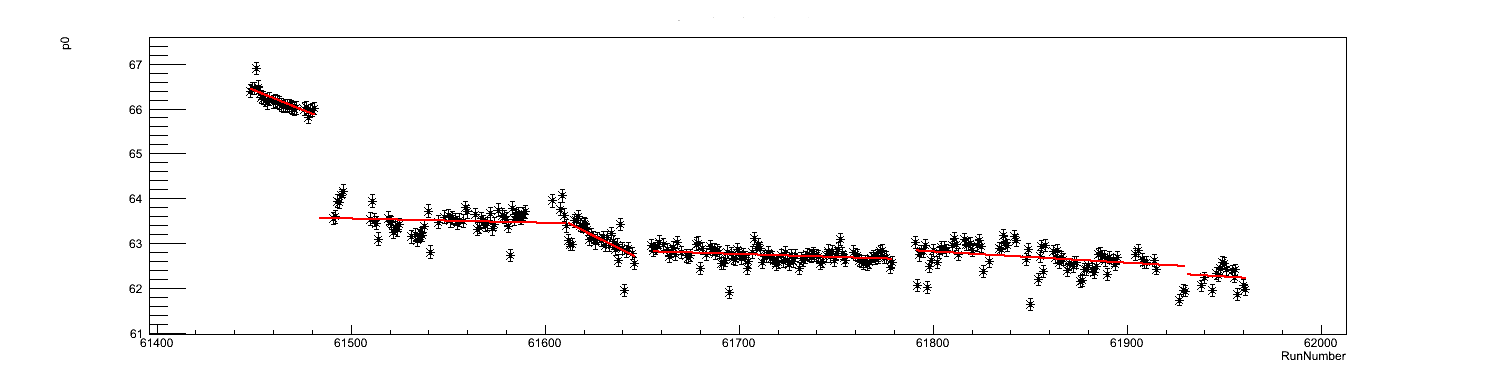
\includegraphics[scale=0.28]{fig_rtpc/p0_RunNumber.png}
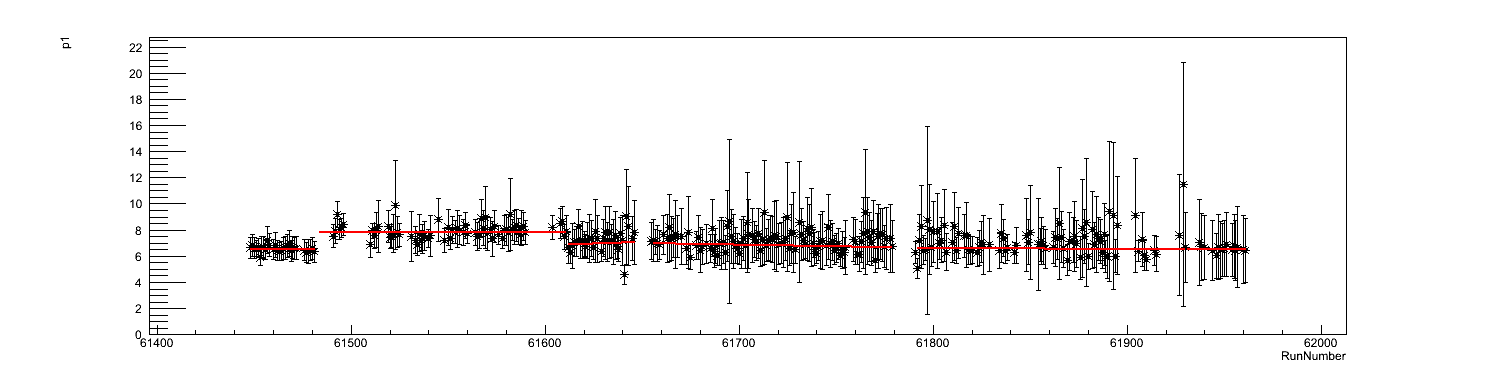
\includegraphics[scale=0.28]{fig_rtpc/p1_RunNumber.png}
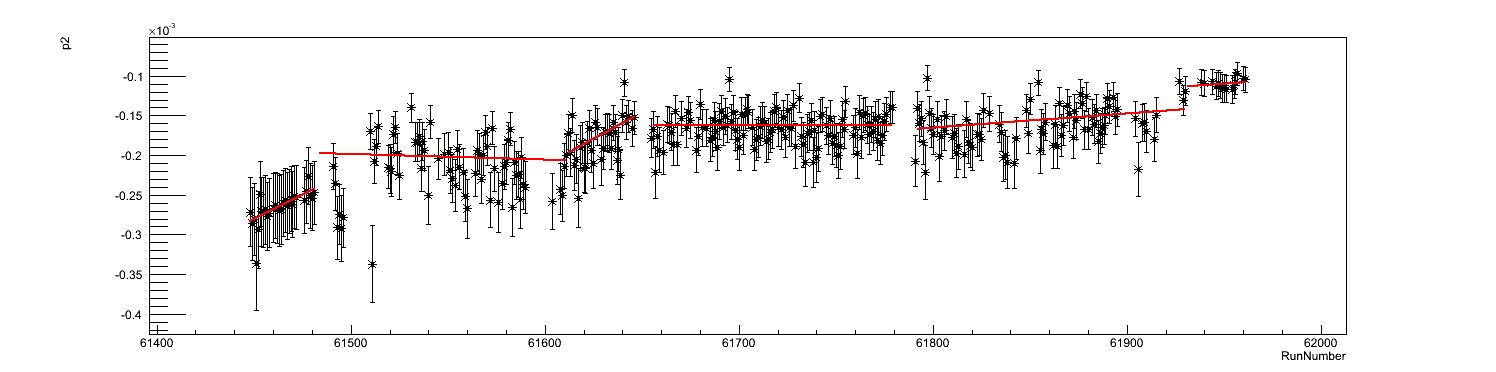
\includegraphics[scale=0.28]{fig_rtpc/p2_RunNumber.png}
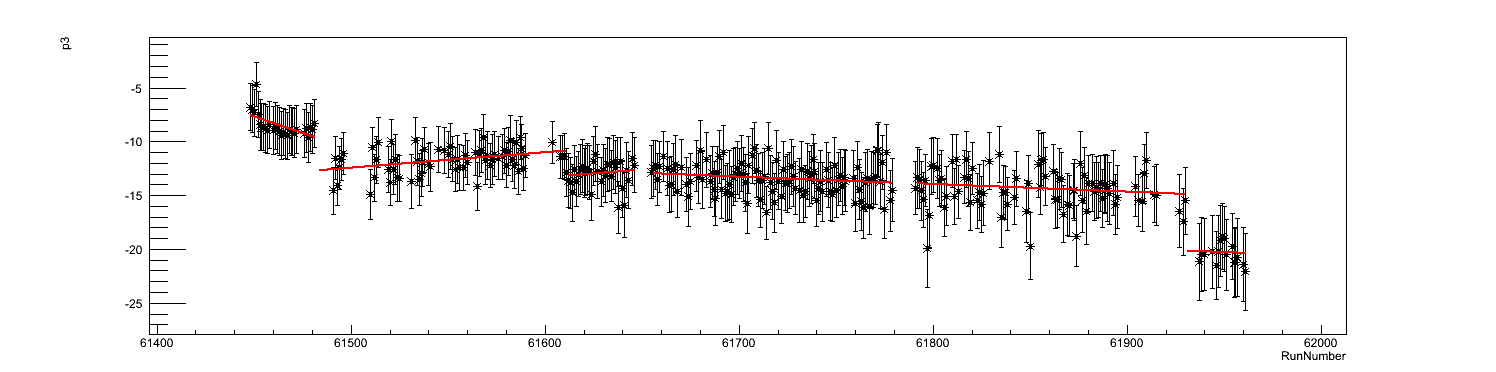
\includegraphics[scale=0.28]{fig_rtpc/p3_RunNumber.png}
\caption{ The fit parameters: $p_{0}$, $p_{1}$, $p_{2}$, and $p_{3}$ for the individual runs. The red lines represent their piece-wise fits. }
\label{fig:Drift_speed_fit_par}
\end{figure} 


\begin{equation}
TDC_{max/2} (z)= p_{0} +  p_{1} * e^{p_{2}*(z-p_{3})^{2}}
\end{equation}

\begin {table}[!h]
\begin{center}
\begin{tabular}{|l|l|l|l|l|}
\hline
run range &  $p_{0}$ &  $p_{1}$ \\&  $p_{2}$ &  $p_{3}$ \\
\hline
61448 - 61481 & 
\small{ 1.14312e+03 - 1.75217e-02 *$r_{N}$} & 
\small{ 3.27339e+00 + 5.32577e-05 *$r_{N}$} \\&
\small{-7.55131e-02 + 1.22429e-06 *$r_{N}$} &  
\small{ 3.76627e+03 - 6.14148e-02 *$r_{N}$}\\
\hline
61483 - 61611 &  
\small{ 1.21405e+02 - 9.40705e-04 *$r_{N}$} & 
\small{ 3.89644e+00 + 6.33813e-05 *$r_{N}$}  \\& 
\small{ 4.09308e-03 - 6.97839e-08 *$r_{N}$} & 
\small{-9.04583e+02 + 1.45062e-02 *$r_{N}$}\\
\hline
61612 - 61646 & 
\small{ 1.39733e+03 - 2.16496e-02 *$r_{N}$} & 
\small{-3.07845e+02 + 5.10814e-03 *$r_{N}$}  \\&
\small{-8.23774e-02 + 1.33384e-06 *$r_{N}$} & 
\small{-9.05752e+02 + 1.44872e-02 *$r_{N}$}\\
\hline
61655 - 61779 &
\small{ 1.45093e+02 - 1.33438e-03 *$r_{N}$} &
\small{ 1.63746e+02 - 2.54273e-03 *$r_{N}$} \\&
\small{-5.10501e-04 + 5.64359e-09 *$r_{N}$} &
\small{ 4.26282e+02 - 7.12408e-03 *$r_{N}$}\\
\hline
61791 - 61930&
\small{ 2.18243e+02 - 2.51495e-03 *$r_{N}$} &
\small{ 4.92691e+01 - 6.90443e-04 *$r_{N}$} \\&
\small{-1.11909e-02 + 1.78407e-07 *$r_{N}$} &
\small{ 4.26297e+02 - 7.12383e-03 *$r_{N}$}\\
\hline
61931 - 61961)&
\small{ 2.18152e+02 - 2.51641e-03 *$r_{N}$} &
\small{ 4.92921e+01 - 6.90070e-04 *$r_{N}$} \\&
\small{-1.11766e-02 + 1.78639e-07 *$r_{N}$} &
\small{ 4.23668e+02 - 7.16628e-03 *$r_{N}$} \\
\hline
\end{tabular}
\caption[]{The parameters of $TDC_{max/2}$ used in EG6 experiment reconstruction codes.}
\label{Table:TDCmax}
\end{center}
\end{table}

~\newpage
\item Drift paths' parametrization:
\begin{equation}
  \Delta \phi (TDC, z)=  \sum\limits_{i=0}^{4} p_{i}(z)*TDC^{i}
\end{equation}
\begin{table}[!h]
\begin{center}
\begin{tabular}{|l|l|l|l|}
\hline
Parameter & ~~~~~constant & ~~~~~~~*z & ~~~~~~~*$z^{2}$\\
\hline
~~~~$p_{0}$   & 0.14222     &-6.52562e-05 & 4.06768e-06\\
\hline
~~~~$p_{1}$   &-0.00147368  & 5.64924e-06 &-7.31944e-07\\
\hline
~~~~$p_{2}$   & 0.000216222 & 6.25749e-09 & 1.8923e-08 \\
\hline
~~~~$p_{3}$   &-3.82450e-06 &-6.29825e-09 &-1.89627e-10\\
\hline
~~~~$p_{4}$   & 3.22973e-08 & 7.52017e-11 & 1.08564e-12\\
\hline
\end{tabular}
\caption{The drift paths extracted in the EG6 experiment.}
\label{table:drift_paths}
\end{center}
\end{table}

\end{itemize}

%\part{SIDIS generalized cross section}
%\begin{align}
%\lefteqn{\frac{d\sigma}{dx \, dy\, d\phi_{S} \,dz\, d\phi_h\, d P_{h\perp}^2}
%=}
%\nonumber \\ & \quad 
%\frac{\alpha^2}{x y Q^2}\,
%\frac{y^2}{2\,(1-\varepsilon)}\,  \biggl( 1+\frac{\gamma^2}{2x} \biggr)\, \Biggl\{ F_{UU ,T} +  %\varepsilon F_{UU ,L} + \sqrt{2\,\varepsilon (1+\varepsilon)}\,\cos\phi_h\,
%F_{UU}^{\cos\phi_h} \nonumber \\  & \quad \qquad + \varepsilon \cos(2\phi_h)\, 
%F_{UU}^{\cos 2\phi_h} + \lambda_e\, \sqrt{2\,\varepsilon (1-\varepsilon)}\,  \sin\phi_h\, 
%F_{LU}^{\sin\phi_h} \phantom{\Bigg[ \Bigg] }
%\nonumber \\  & \quad \qquad + S_\parallel\, \Bigg[ \sqrt{2\, \varepsilon (1+\varepsilon)}\,
%  \sin\phi_h\, F_{UL}^{\sin\phi_h} +  \varepsilon \sin(2\phi_h)\,  F_{UL}^{\sin 2\phi_h} \Bigg]
%\nonumber \\  & \quad \qquad
%+ S_\parallel \lambda_e\, \Bigg[ \, \sqrt{1-\varepsilon^2}\; 
%F_{LL} +\sqrt{2\,\varepsilon (1-\varepsilon)}\,
%  \cos\phi_h\,  F_{LL}^{\cos \phi_h} \Bigg] \nonumber \\  & \quad \qquad
%+ |{S}_\perp|\, \Bigg[ \sin(\phi_h-\phi_S)\, \Bigl(F_{UT ,T}^{\sin(\phi_h -\phi_S)}
%+ \varepsilon\, F_{UT ,L}^{\sin(\phi_h -\phi_S)}\Bigr) \nonumber \\  & \quad  \qquad \qquad
%+ \varepsilon\, \sin(\phi_h+\phi_S)\,  F_{UT}^{\sin(\phi_h +\phi_S)}
%+ \varepsilon\, \sin(3\phi_h-\phi_S)\, F_{UT}^{\sin(3\phi_h -\phi_S)}
%\phantom{\Bigg[ \Bigg] } \nonumber \\  & \quad \qquad \qquad + \sqrt{2\,\varepsilon (1+\varepsilon)}\, 
%  \sin\phi_S\,  F_{UT}^{\sin \phi_S }
%+ \sqrt{2\,\varepsilon (1+\varepsilon)}\,  \sin(2\phi_h-\phi_S)\,  
%F_{UT}^{\sin(2\phi_h -\phi_S)} \Bigg] \nonumber \\  & \quad \qquad 
%+ |{S}_\perp| \lambda_e\, \Bigg[  \sqrt{1-\varepsilon^2}\, \cos(\phi_h-\phi_S)\, 
%F_{LT}^{\cos(\phi_h -\phi_S)}
%+\sqrt{2\,\varepsilon (1-\varepsilon)}\,   \cos\phi_S\,  F_{LT}^{\cos \phi_S}
%\nonumber \\  & \quad \qquad \qquad +\sqrt{2\,\varepsilon (1-\varepsilon)}\,  \cos(2\phi_h-\phi_S)\,  %F_{LT}^{\cos(2\phi_h - \phi_S)} \Bigg] \Biggr\}
%\label{crossmaster}
%\end{align}

%\begin{align}
%\varepsilon &= \frac{1-y -\frac{1}{4} \gamma^2 y^2}{1-y
%  +\frac{1}{2} y^2 +\frac{1}{4} \gamma^2 y^2} ,
%\end{align}  


\chapter{The parametrization of the IC-photons energy corrections} \label{App:AppendixA}
\begin{itemize}
\item $\alpha$ parametrization
\vspace{-0.2in}
\begin{equation}
\alpha (x) = c_{0} + c_{2} \left[ e^{-c_{3}(x - c_{1})} - e^{-c_{4}(x - c_{1})} \right],
\end{equation}

\vspace{-0.2in}
\begin {table}[!h]
\begin{center}
\begin{tabular}{|l|l|l|l|l|l|l|l|}
\hline
$Fun_{N}$ & xmin  &   xmax    &  $c_{0}$     &   $c_{1}$    &  $c_{2}$      &   $c_{3}$  &   $c_{4}$\\
\hline
1  &  61510    & 61514   &  -0.00671929   &  61493     & -0.00868856    &   -0.114874  &  -0.117953\\
\hline
2   &  61519   &  61525  &    -0.00160398   &  61585.7  &  -2.1e-09    &   0.38362    &  0.38362\\
\hline
3   &  61531   &  61545  &    -0.00956513   &  61876.8  & -0.0295579   &    1.23958e-06 &  0.000704112\\
\hline
4   &  61546   &  61556  &    -0.000414459  &   61521.8  &-0.0179471   &    -0.0316302  &  -0.030899\\
\hline
5   &  61558   &  61580  &    -0.00731749  &   61532.4 &  -0.465254   &    0.0200131   &   0.0193213\\
\hline
6   &  61581   & 61590   &   0.0604759    & 61561.7  & -19.3314    & 0.0407449   & 0.0411026\\
\hline
7   &  61604   & 61608    &  -0.00320342  &   61521.1  &  -0.00074357   &    -0.018373  &    -0.0243743\\
\hline
8   &  61609   & 61622     & -0.00205987  &   61649.1  &   5.94004e-05   &    0.0760846  &    -2.64412\\
\hline
9   &  61623   & 61637    &  -0.00153458  &   61640.7  &   -1.02541e-10 &   0.965545   &   0.959411\\
\hline
10  &   61638   &  61646  &    -0.000735223  &   61763.1  & -0.00476067   & 0.0423013  &    0.0422956\\
\hline
11  &   61655  &  61675   &   -0.00123166   &  61561.1  &  -2.63733e-06  &  -0.159566  &    -0.159566\\
\hline
12  &  61678    & 61711   &   -0.00294886   &  61670.6   & -0.0079126   &    0.052612  &    0.0252883\\
\hline
13   &  61712   &  61713   &   -0.00102705   &  61711.9 &   -0.0034062 &  -3.1972   &   -3.19763\\
\hline
14   &  61714   &  61724   &   -0.00109184   &  61731.2&    -1.14221e-06  &     0.308061   &-4.24803\\
\hline
15   &  61725   &  61729   &   -0.00915958   &  61716.6 &     -0.0240355 &      0.137179  & 0.0524492\\
\hline
16   &  61731   &  61779   &   -0.00295947   &  61669.4 &  0.0130552    & 0.00768358   &   0.0117274\\
\hline
17   &  61791   &  61796   &   -0.00117275   &  61791.9  &  -0.00210188  &  5.63266   &   5.63003\\
\hline
18   &  61797   &  61826   &   0.00155106   &  61787.7 &  -0.980189  &     0.0514066 &     0.0518518\\
\hline
19   &  61829   &  61843   &   -0.0015276  &   61826 &  -0.00204473 &      2.72258   &   0.275824\\
\hline
20   &  61848  &   61874   &   0.0265578   &  61973.2 &  -0.0249309&    0.0010753   &   -0.186452\\
\hline
21   &  61876 &  61895    &  -0.00205642   &  61715.7  & -3.3277e-05 &   -0.065808   &   -0.0658091\\
\hline
22   &  61904  & 61915    &  -0.00274984   &  62178.9  &   -0.107207&     0.00976882  &    0.00977186\\
\hline
23   &  61925   &61930    &  0.0064528    & 61924.8   & -0.00849265  & 0.0278942  &   9.3268 \\
\hline
\end{tabular}
\caption{$\alpha$ parametrization shown in figure \ref{fig:ic_alpha_beta_fitting}.}
\label{Table:ic_alpha_corrections}
\end{center}
\end{table}

~\newpage
\item $\beta$ parametrization

\begin{equation}
\beta (x) = p_{0} + p_{2} \left[ e^{-p_{3}(x - p_{1})} - e^{-p_{4}(x - p_{1})} \right],
\end{equation}

\begin {table}[!h]
\begin{center}
\begin{tabular}{|l|l|l|l|l|l|l|l|}
\hline
$Fun_{N}$ & xmin  &   xmax    &  $p_{0}$     &   $p_{1}$    &  $p_{2}$      &   $p_{3}$  &   $p_{4}$\\
\hline
1   &  61510   &61514   &   0.139127   &  61508.7   &   -0.00705827      & -0.127   &   -0.163719\\
\hline
2   &  61519   &  61525  &    0.144057  &   61553.1  &    6.44528e-05   &    0.384066 &     0.384069\\
\hline
3   &  61531   &  61545   &   -0.238301    & 61487    &  -1.28623      & 0.0260483   &   0.011476\\
\hline
4   &  61546    & 61556    &  0.0904474   &  61545.1   &   -0.0367149 &      2.10481  &    -0.0186192\\
\hline
5   &  61558  &   61580     & 0.095243   &  61543.5  &    -0.197639  &     0.0280817  &    0.015222\\
\hline
6   &  61581   &  61590 & 0.0643454     &61557.1    &  -0.394422    &   0.0358816   &   0.0212999\\
\hline
7   &  61604    & 61608  &    0.138436 &    61605.4  &    -0.0142253    &   -0.0323464  &    -0.0103419\\
\hline
8  &   61609    & 61622   &   0.135047    & 61605.8   &   -0.00856825    &   0.157423    &  0.0474859\\
\hline
9   &  61623    & 61637    &  0.137445   &  61646.8    &  -1.46307e-05  &     0.273975  &    -0.0770047\\
\hline
10 &    61638    & 61646    &  0.141909 &    61651.9 &     -0.103873    &   0.00713496   &  0.000949948\\
\hline
11&   61655  & 61675  & 0.127712   &  61652.8   &  -0.00969769     &  0.220956  &    0.00215349\\
\hline
12 &  61678   &  61711 &     0.137774     &61697.7  &    -9.15967e-05    &   0.237965 &     -0.158587\\
\hline
13  & 61712   & 61713   &   0.124706     &61655.1    &  -3.72443e-05    &   -0.0443564 &     -0.100321\\
\hline
14    & 61714  &   61724 &     0.138057 &    61726.8  &    -0.000274029   &    0.234    &  -4.45937\\
\hline
15   &  61725  &   61729  &    0.108381    & 61721.3   &   -0.0289603    &   0.77633  &    -0.00285553\\
\hline
16  &   61731  &   61779   &   0.113727   &  61726   &   -0.0236114     &  0.243927    &  -0.00196355\\
\hline
17 &    61791  &   61791    &  0.136619  &   0.0   &   0.0   &    0.0  &    0.0\\
\hline
18&   61792   &  61796 & 0.138708   &  61914.5   &   1.07991e-09     &  0.181595    &  0.181612\\
\hline
19 &  61797  &   61825  &    0.137559   &  61839.6 &     -0.000312349  &     0.160791&      0.159434\\
\hline
20  &61826   & 61843     & 0.0359758   &  61810.5   &   -0.10032      & 0.215911     & -0.000529924\\
\hline
21 & 61848  &  61874      &0.116396   &  61891.7   &   -0.385562     &  -0.0563216    &  -0.0479573\\
\hline
22&   61876  &   61915  &  0.105816  &   61872.2    &  -0.0312028     &  0.384691    &  -0.00145868\\
\hline
23 & 61925   &  61930    &  0.137809   &  61927.5    &  -0.00071665  &     0.620419   &   0.222406\\

\hline
\end{tabular}
\caption{$\beta$ parametrization shown in figure \ref{fig:ic_alpha_beta_fitting}.}
\label{Table:ic_beta_corrections}
\end{center}
\end{table}
\end{itemize}

~\newpage

\chapter{Exclusive $\pi^{0}$ events selection}\label{app:Exclusive_pi0_selection}

The exclusive selection of the experimental $e^{4}He\pi^{0}$ and $ep\pi^{0}$ events require the detection of only one good electron, one good $\pi^{0}$ in the topology ICIC or ICEC, and one good $^{4}He$ track in the coherent channel or one good proton in the incoherent channel case. Furthermore, in order to ensure that this is a deep process we apply a set of initial requirements. The exclusivity of the reaction is ensured by a set of exclusivity cuts like for the DVCS channels. These requirements and exclusivity cuts are presented for the case of the coherent $e^{4}He\pi^{0}$ events are:

\paragraph{Initial criteria} ~\\
These requirements are made to ensure that the selected events occurre at the partonic level:
\begin{itemize}
\item High virtuality of the exchanged photon ($Q^{2}$>1 $GeV^{2}$).
\item High energy of the emitted $\pi^{0}$ ($E_{\pi^{0}}$ > 2 GeV).
\item The invariant mass of the virtual photon and the target proton is greater than 2 GeV$^{2}$/c$^{2}$ in order to avoid the baryons resonances region.
\item The transfer momentum squared ($-t$) between the initial target and the recoil one is greater than the minimum allowed one ($t_{min}$) defined by the kinematics of the incoming and the scattered electrons. The definition of $t_{min}$ for each channel can be found in the corresponding DVCS channel selection presented previously.
\end{itemize}

\paragraph{Exclusivity requirements}
~\\
~\\The exclusivity of the selected $e^{4}He\pi^{0}$ events is done with the following cuts:
\begin{itemize}
\item The coplanarity cut ($\Delta \phi$) between the recoil $^{4}He$ and the produced $\pi^{0}$.
\item The missing energy, mass and transverse momentum cuts in the configuration $e^{4}He\pi^{0}X$.
\item The missing mass cut in the configuration $e^{4}HeX$.
\item The missing mass cut in the configuration $e\pi^{0}X$.
\item The cone angle cut between $e^{4}HeX$ and the reconstructed $\pi^{0}$.
\end{itemize}
  The same procedure holds for the case of the incoherent $ep\pi^{0}$ events. In the following two subsections, the results of the two channels selection are presented.
~\newpage
\section{$e^{4}He\pi^{0}$ exclusivity cuts}
The events which pass the following exclusivity cuts are assumed to be good $e^{4}He\pi^{0}$ events.

\begin{figure}[h!]
\centering
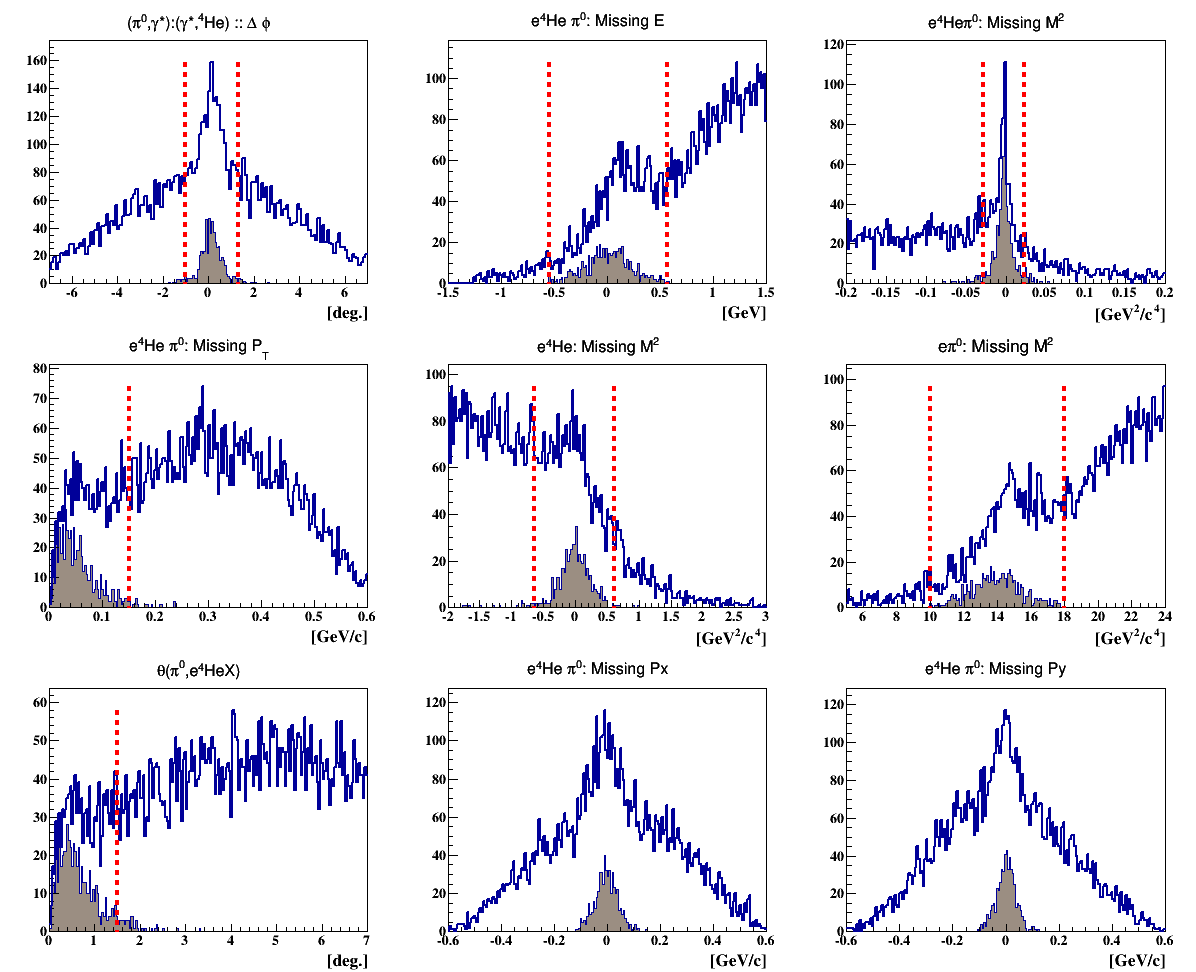
\includegraphics[scale=0.4]{fig_dvcs/all_coh_pi0_exc_cuts.png}
\caption{The blue distributions represent all the  $e^{4}He\pi^{0}$ events before the exclusivity cuts. The shaded distributions show the events which passed all the exclusivity cuts except for the quantity plotted. The red lines are $3\sigma$ cuts. The mean and sigma values of each distribution are listed in table \ref{Table:cohpi0_exclusivity_cuts}.} 
\label{fig:cohpi0_exclusivty_cuts}
\end{figure}

\paragraph{Comparison with simulation}
~\\
~\\As for the selection of the experimental $e^{4}He\pi^{0}$ events, the simulated events have to pass an equivalent set of exclusivity cuts in addition to the $\pi^{0}$ electroproduction criteria, presented at the beginning of this section. In this section, we show the comparison between the experimental and the simulated selected  $e^{4}He\pi^{0}$ events as a function of the kinematic variables ($Q^{2}$, $x_{B}$, $-t$), figure \ref{fig:coh_pi0_comparison_with_simulation}, and as a function of the variables used for the exclusivity cuts, figure \ref{fig:coh_pi0_comparison_with_simulation_2}.\\

\begin{figure}[h!]
\hspace{-0.1in}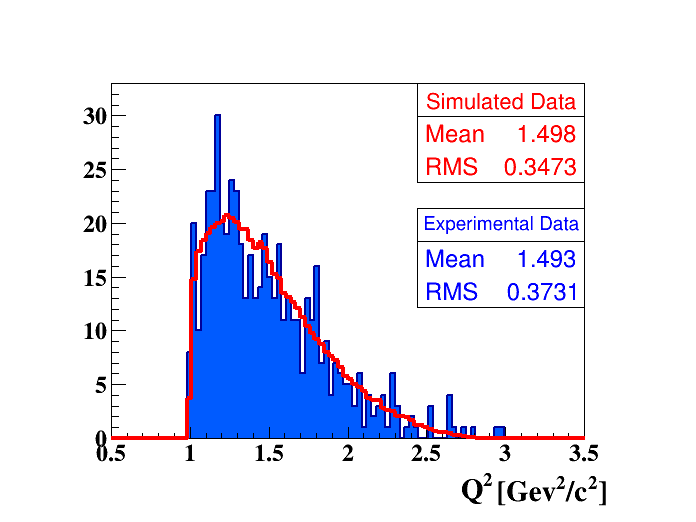
\includegraphics[scale=0.37]{fig_dvcs/comp/Q2_Coh_pi0.png}
\hspace{-0.4in}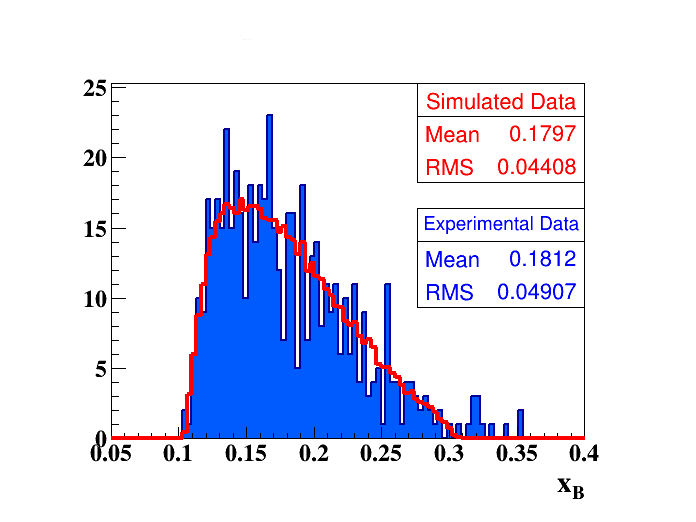
\includegraphics[scale=0.37]{fig_dvcs/comp/xB_Coh_pi0.png}
\hspace*{-0.1in}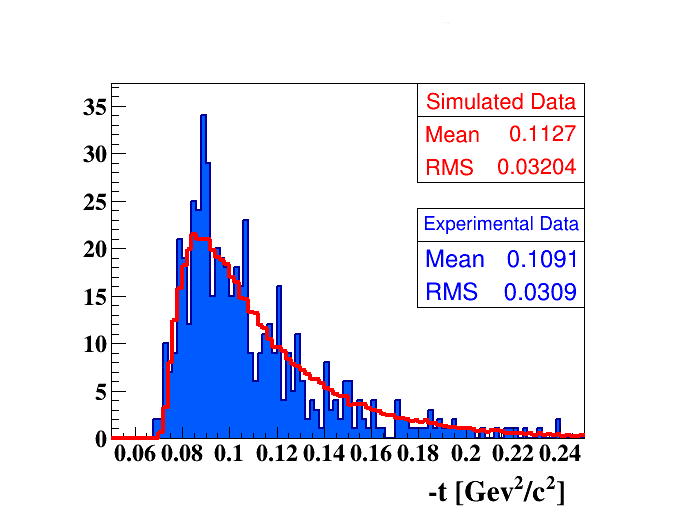
\includegraphics[scale=0.37]{fig_dvcs/comp/t_Coh_pi0.png}
\hspace{-0.4in}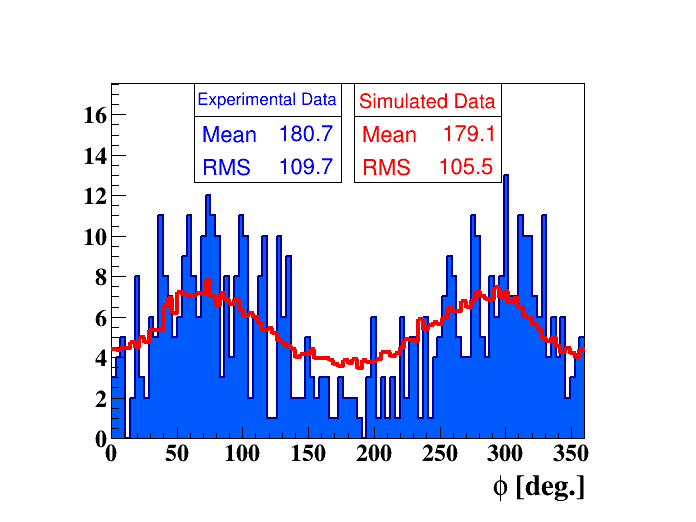
\includegraphics[scale=0.37]{fig_dvcs/comp/phi_h_Coh_pi0.png}
\caption{Comparison between the simulated $e^{4}He\pi^{0}$ events (red lines) and the experimental events (blue shaded distributions) as a function of the kinematic variables: $Q^{2}$, $x_{B}$, $-t$ and $\phi_{h}$ respectively from top to right to right and from top to bottom.}
\label{fig:coh_pi0_comparison_with_simulation}
\end{figure}

\begin{figure}[h!]
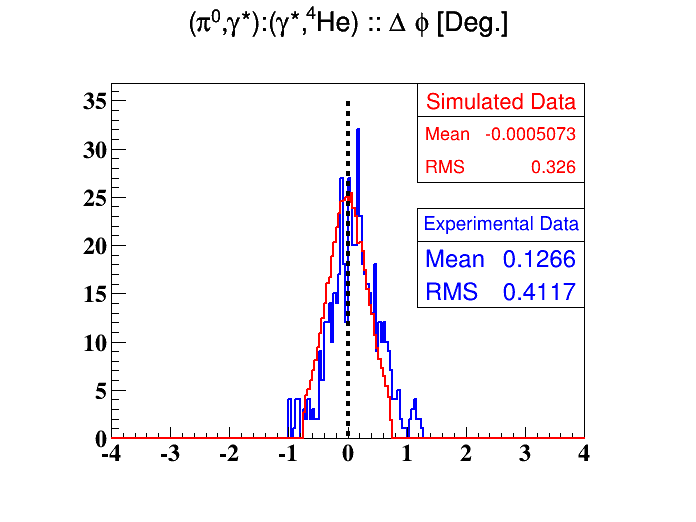
\includegraphics[scale=0.35]{fig_dvcs/comp/Coh_pi0_delta_phi.png}
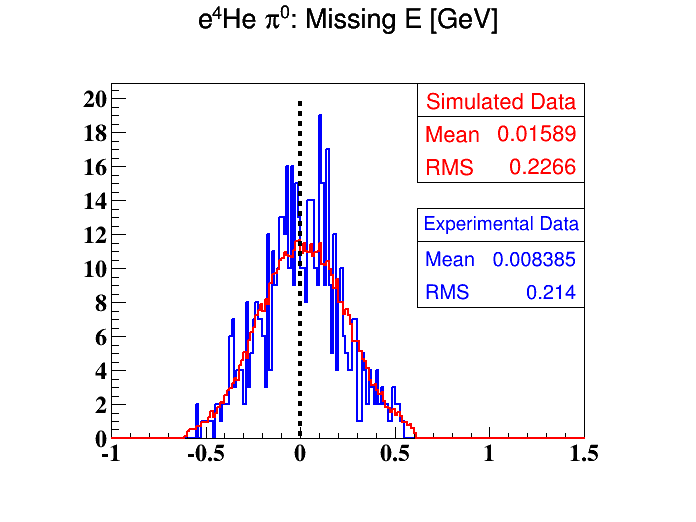
\includegraphics[scale=0.35]{fig_dvcs/comp/Coh_pi0_e4Hepi0_E_Mis.png}
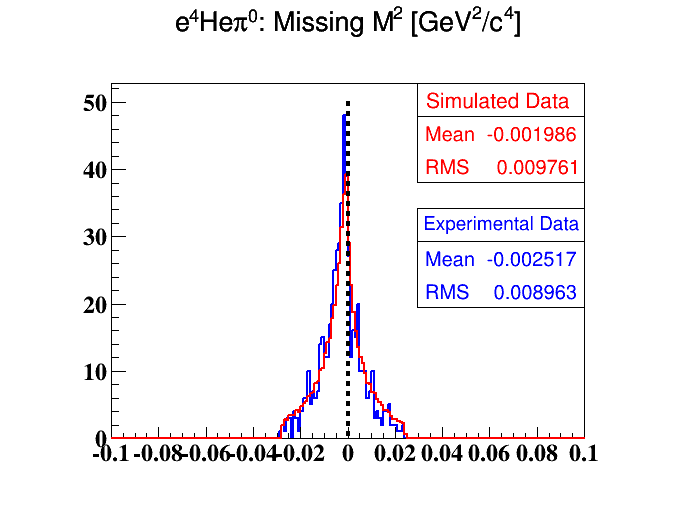
\includegraphics[scale=0.35]{fig_dvcs/comp/Coh_pi0_e4Hepi0_M2_Mis.png}
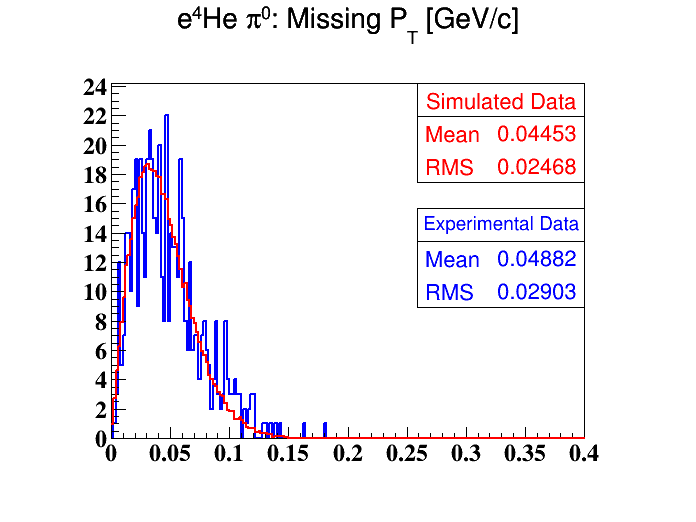
\includegraphics[scale=0.35]{fig_dvcs/comp/Coh_pi0_e4Hepi0_PT_Mis.png}
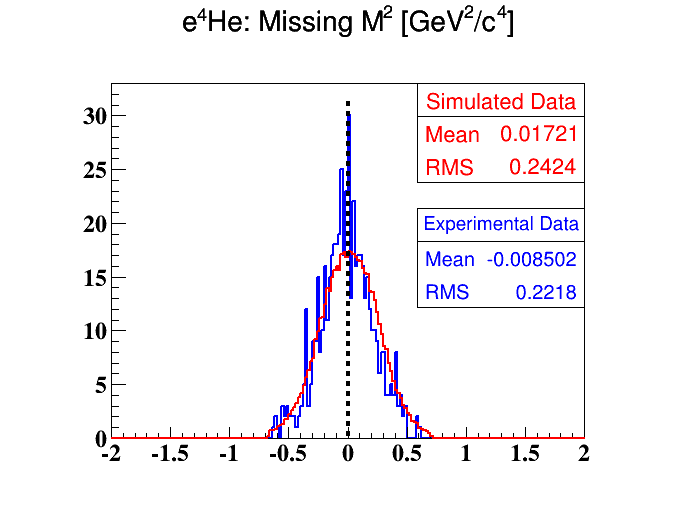
\includegraphics[scale=0.35]{fig_dvcs/comp/Coh_pi0_e4He_M2_Mis.png}
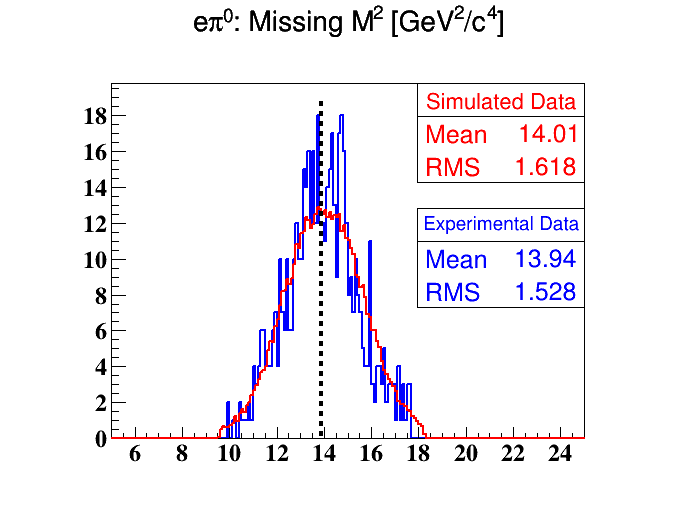
\includegraphics[scale=0.35]{fig_dvcs/comp/Coh_pi0_epi0_M2_Mis.png}
\caption{Comparison between the simulated and experimental $e^{4}He\gamma$ events in terms of the exclusivity variables. The vertical black line indicates the theoretically expected value for each exclusive variable.} 
\label{fig:coh_pi0_comparison_with_simulation_2}
\end{figure}

Even with low experimental statistics, figures \ref{fig:coh_pi0_comparison_with_simulation} and \ref{fig:coh_pi0_comparison_with_simulation_2} show a good match between the simulation and the experimental   $e^{4}He\gamma$ events for the different kinematic variables, which is satisfying  for our background subtraction goal. 


~\newpage
~\newpage
\section{$ep\pi^{0}$ exclusivity cuts}
The $ep\pi^{0}$ events which pass the initial deepness criteria and the exclusivity cuts, marked by the red vertical lines in the figure below, are considered as clean events.

\begin{figure}[h!]
\centering
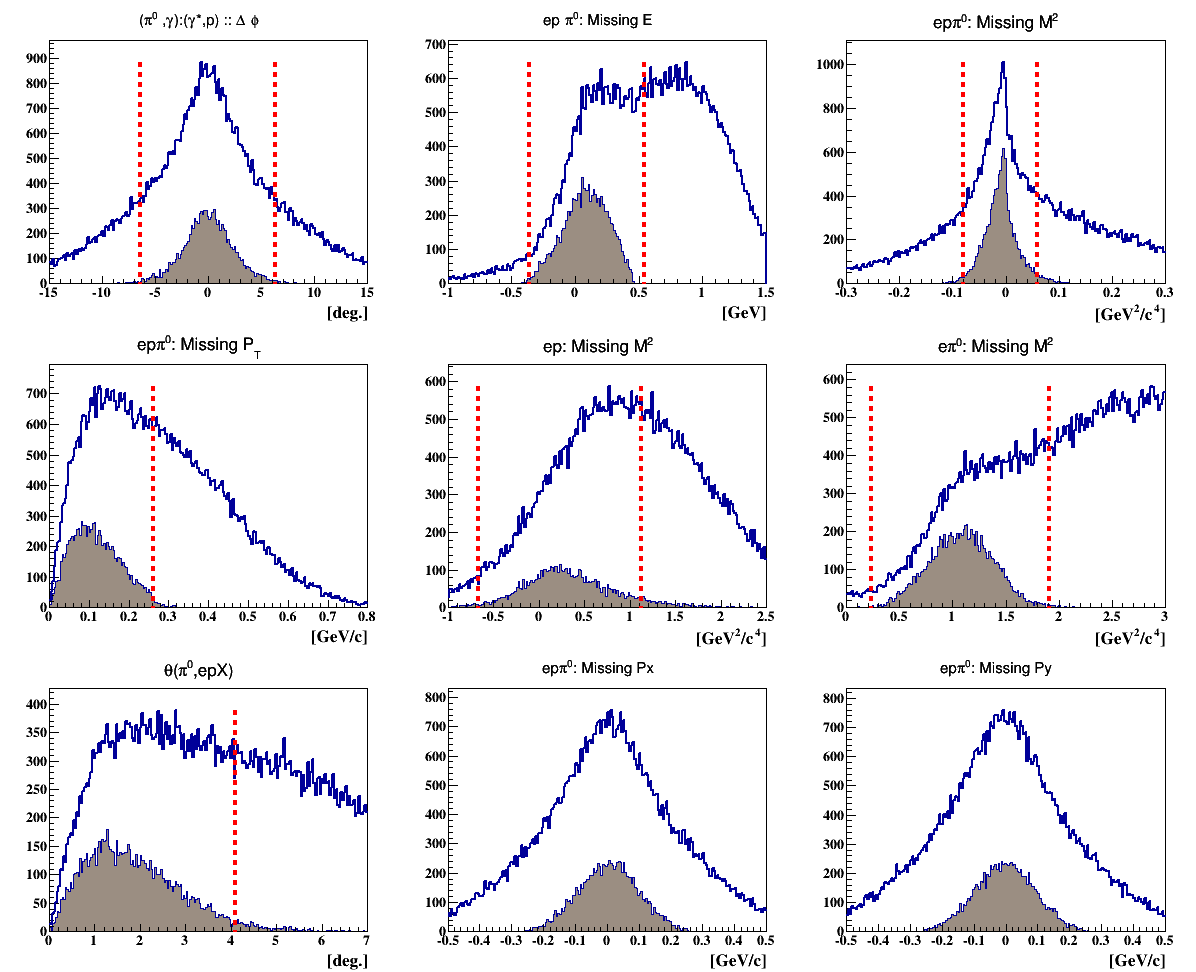
\includegraphics[scale=0.4]{fig_dvcs/all_incoh_pi0_exc_cuts.png}
\caption{The blue distributions represent all the $ep\pi^{0}$ events before any exclusive requirement. The shaded brown distributions show the events which passed all the exclusivity cuts except the quantity plotted. The vertical red lines represent $3\sigma$ cuts on the shaded distribution. The mean and sigma values of each distribution are listed in table \ref{Table:incohpi0_exclusivity_cuts}.} 
\label{fig:incohpi0_exclusivty_cuts}
\end{figure}



\paragraph{Comparison with simulation}
~\\
~\\
In this section, the experimental selected $ep\pi^{0}$ events are compared to the Monte Carlo simulated events. Figure \ref{fig:incoh_pi0_comparison_with_simulation} shows the comparison as a function of the kinematic variables. Figure \ref{fig:incoh_comparison_with_simulation_exclusive} shows the comparison in terms of the different exclusivity variables. One can see an agreement within some degrees of differences, which might come from the fact that our protons are bound ones and the physics of the nuclear process is not fully understood. 
\begin{figure}[h!]
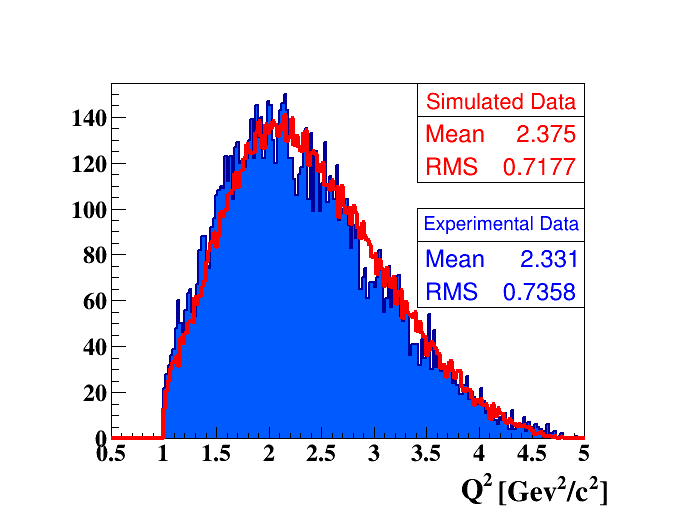
\includegraphics[scale=0.35]{fig_dvcs/comp/Q2_InCoh_pi0.png}
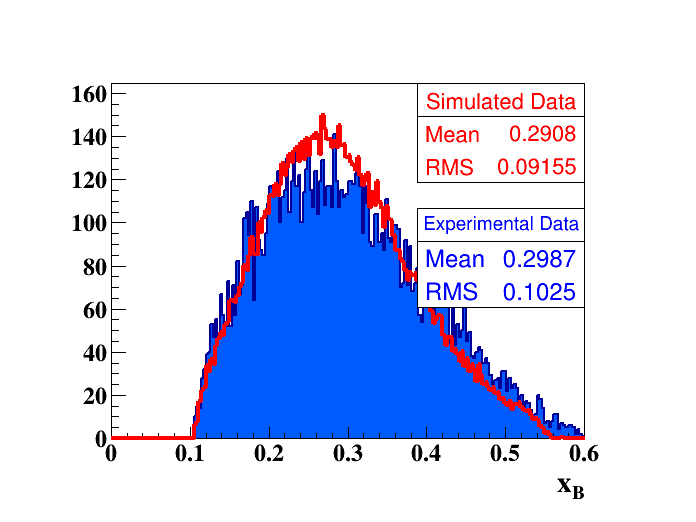
\includegraphics[scale=0.35]{fig_dvcs/comp/xB_InCoh_pi0.png}
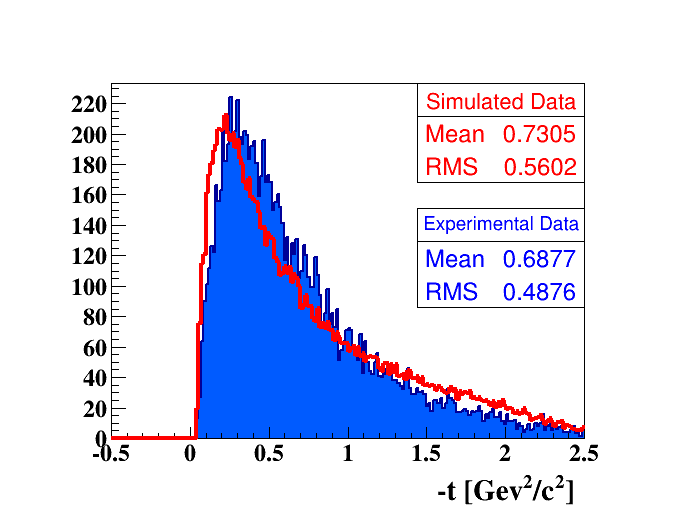
\includegraphics[scale=0.35]{fig_dvcs/comp/t_InCoh_pi0.png}
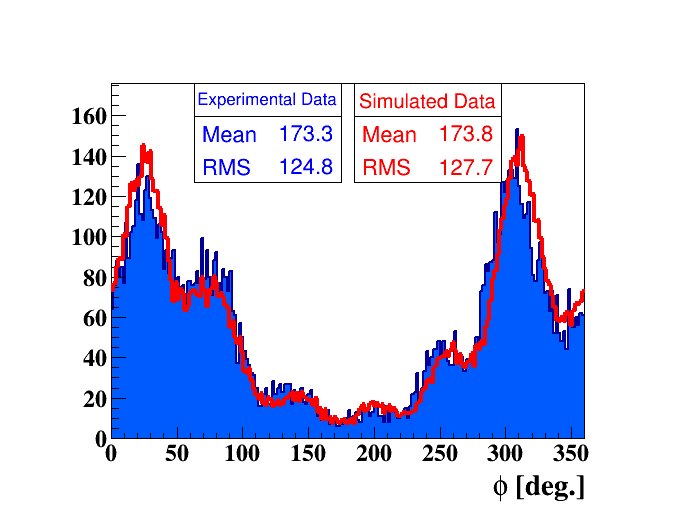
\includegraphics[scale=0.35]{fig_dvcs/comp/phi_h_InCoh_pi0.png}
\caption{Comparison between the Monte Carlo simulated $ep\pi^{0}$ events (red lines) and the experimental ones (blue shaded distributions) as a function of the kinematic variables: $Q^{2}$, $x_{B}$, $-t$, and $\phi$, respectively from top to right to right and from top to bottom.}
\label{fig:incoh_pi0_comparison_with_simulation}
\end{figure}

\begin{figure}[h!]
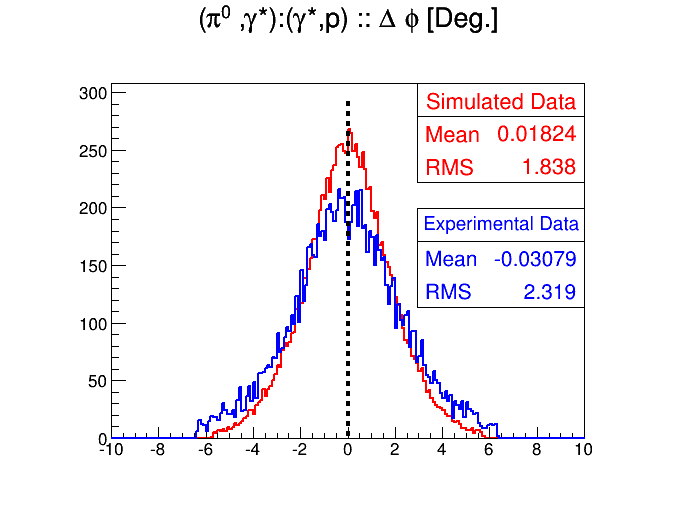
\includegraphics[scale=0.35]{fig_dvcs/comp/InCoh_pi0_delta_phi_InCoh.png}
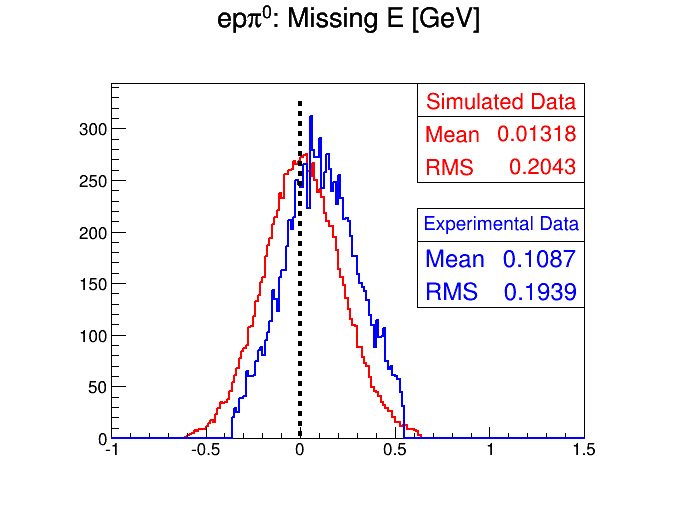
\includegraphics[scale=0.35]{fig_dvcs/comp/InCoh_pi0_eppi0_E_Mis.png}
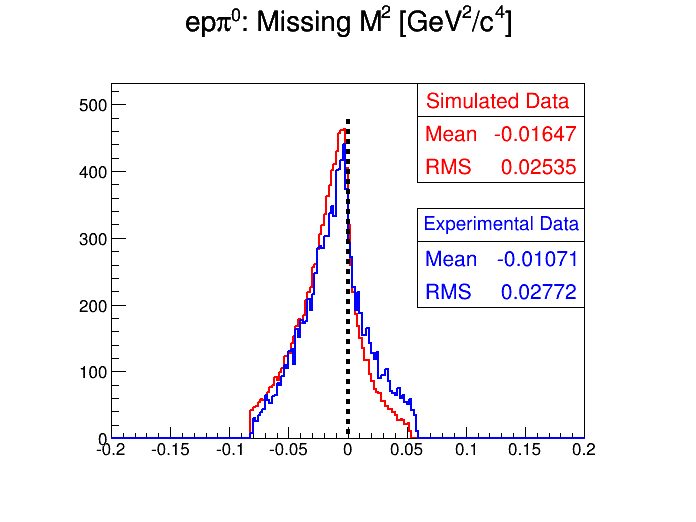
\includegraphics[scale=0.35]{fig_dvcs/comp/InCoh_pi0_eppi0_M2_Mis.png}
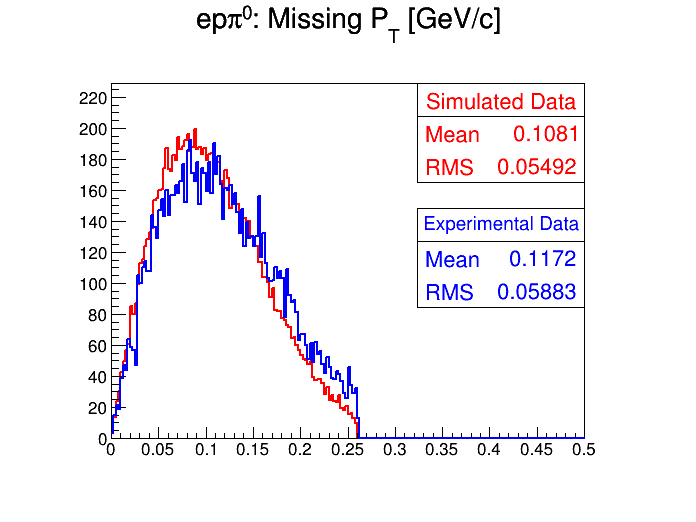
\includegraphics[scale=0.35]{fig_dvcs/comp/InCoh_pi0_eppi0_PT_Mis.png}
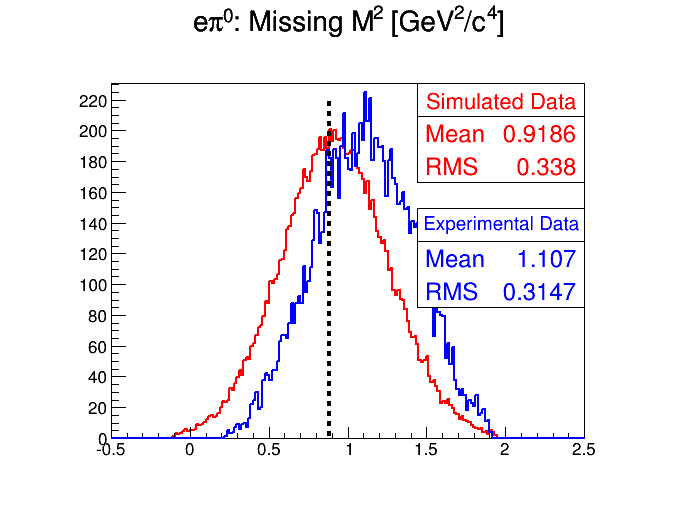
\includegraphics[scale=0.35]{fig_dvcs/comp/InCoh_pi0_epi0_M2_Mis_InCoh.png}
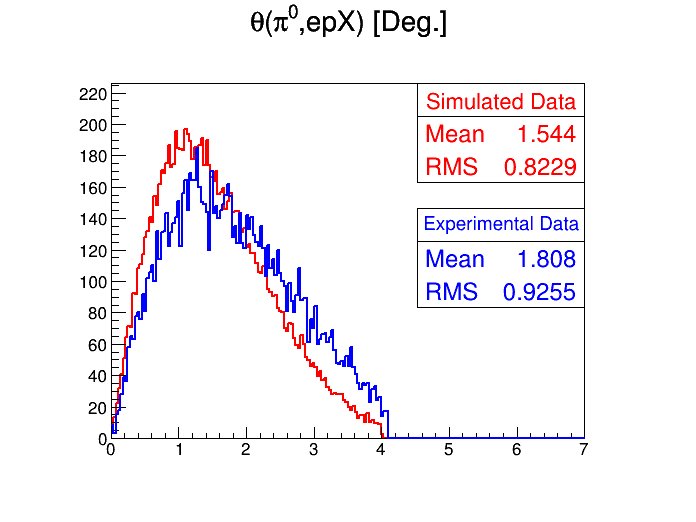
\includegraphics[scale=0.35]{fig_dvcs/comp/InCoh_pi0_Theta_pi0X_InCoh.png}
\caption{Comparison between the simulated and experimental $ep\pi^{0}$ DVCS events as a function of the variables used for the exclusivity cuts. The simulated distributions are normalized with respect to the experimental ones. The vertical black lines indicate the theoretically expected values.} 
\label{fig:incoh_comparison_with_simulation_exclusive}
\end{figure}


\chapter{Tables list of the exclusive distributions}\label{exclusivity_cuts}
\begin{itemize}

\item Exclusive $e^{4}He\gamma$ distributions
\begin {table}[!h]
\begin{center}
\begin{tabular}{|l|l|l|}
\hline
The quantity &  ~~~mean & ~~~~~$\sigma$ \\
\hline
$\Delta \phi$ &  1.86020e-01 & 4.64936e-01 \\
\hline
$E_{X}$ ($e^{4}He\gamma X$) &  1.48023e-02 & 2.51854e-01 \\ 
\hline
$M^{2}_{X}$ ($e^{4}He\gamma X$) &  -2.98662e-03 & 9.28645e-03 \\ 
\hline
$pt_{X}$ ($e^{4}He\gamma X$) & 4.14664e-02 & 4.24914e-02 \\ 
\hline
$M^{2}_{X}$ ($e^{4}HeX$) & -3.45128e-02 & 2.28247e-01 \\
\hline
$M^{2}_{X}$ ($e\gamma X$) & 1.39930e+01 & 1.61245 \\
\hline
$\theta$ ($\gamma$,$e^{4}HeX$) &  5.08070e-01 & 4.74883e-01\\
\hline
$px_{X}$ ($e^{4}He\gamma X$) & -2.32102e-03  & 4.52945e-02\\
\hline
$py_{X}$ ($e^{4}He\gamma X$) &  -8.97351e-04 & 3.89937e-02\\ 
\hline
\end{tabular}
\caption{ The mean and sigma values of the exclusive coherent quantities drawn in figure \ref{fig:coh_exclusivty_cuts}.}
\label{Table:coh_exclusivity_cuts}
\end{center}
\end{table}


\item Exclusive $e^{4}He\pi^{0}$ distributions
\begin {table}[!h]
\begin{center}
\begin{tabular}{|l|l|l|}
\hline
The quantity &  ~~~mean & ~~~~~$\sigma$  \\
\hline
$\Delta \phi$ & 1.41750e-01  & 3.84202e-01 \\
\hline
$E_{X}$ ($e^{4}He\pi^{0} X$)     &  7.80328e-03 & 1.85770e-01 \\
\hline
$M^{2}_{X}$ ($e^{4}He\pi^{0} X$) &  -2.31650e-03 & 8.65851e-03 \\
\hline
$pt_{X}$ ($e^{4}He\pi^{0} X$)    & 4.36619e-02  & 3.25254e-02 \\
\hline
$M^{2}_{X}$ ($e^{4}HeX$) &  -1.30346e-02 & 2.07791e-01 \\
\hline
$M^{2}_{X}$ ($e\pi^{0} X$)  & 1.39835e+01 & 1.33781\\
\hline
$\theta$ ($\pi^{0}$,$e^{4}HeX$) & 5.30001e-01  & 3.44745e-01\\
\hline
$px_{X}$ ($e^{4}He\pi^{0} X$)    &   -3.79596e-03  &  4.20732e-02\\
\hline
 $py_{X}$ ($e^{4}He\pi^{0} X$)    &   9.41010e-04  & 3.50393e-02 \\
\hline
\end{tabular}
\caption{ The mean and sigma values of the exclusive coherent quantities drawn in figure \ref{fig:cohpi0_exclusivty_cuts}.}
\label{Table:cohpi0_exclusivity_cuts}
\end{center}
\end{table}


~\newpage
\item Exclusive $ep\gamma$ distributions

\begin {table}[!h]
\begin{center}
\begin{tabular}{|l|l|l|}
\hline
The quantity &  ~~~mean & ~~~~~$\sigma$ \\
\hline
$\Delta \phi$ &  4.22584e-02 & 1.39413 \\
\hline
$E_{X}$ ($ep\gamma X$) &  6.27739e-02 & 1.34499e-01 \\
\hline
$M^{2}_{X}$ ($ep\gamma X$) &  -1.00889e-02 & 1.58503e-02 \\ 
\hline
$pt_{X}$ ($ep\gamma X$) & 8.03008e-02 & 4.28511e-02 \\  
\hline
$M^{2}_{X}$ ($epX$) &  2.40257e-01 & 3.66321e-01 \\
\hline
$M^{2}_{X}$ ($e\gamma X$) &  1.01266 & 2.03835e-01 \\
\hline
$\theta$ ($\gamma$, $epX$) &  1.06788 & 6.76469e-01 \\
\hline
$px_{X}$ ($ep\gamma X$) & 3.48024e-03  &  8.19527e-02\\
\hline
$py_{X}$ ($ep\gamma X$) & -1.50911e-03 & 8.16219e-02\\
\hline
\end{tabular}
\caption{ The mean and sigma values of the exclusive incoherent quantities drawn in figure \ref{fig:incoh_exclusivty_cuts}.}
\label{Table:incoh_exclusivity_cuts}
\end{center}
\end{table}


\item Exclusive $ep\pi^{0}$ distributions
\begin {table}[!h]
\begin{center}
\begin{tabular}{|l|l|l|}
\hline
The quantity &  ~~~mean & ~~~~~$\sigma$  \\
\hline
$\Delta \phi$ & -3.25864e-02  & 2.11499 \\ 
  
\hline
$E_{X}$ ($ep\pi^{0} X$) &  9.23934e-02 & 1.50977e-01 \\
  
\hline
$M^{2}_{X}$ ($ep\pi^{0} X$) &  -1.11900e-02 & 2.31963e-02 \\
  
\hline
$pt_{X}$ ($ep\pi^{0} X$) & 1.02247e-01 & 5.31387e-02 \\
  
\hline
$M^{2}_{X}$ ($epX$) & 2.27334e-01  & 2.98775e-01\\
\hline
$M^{2}_{X}$ ($e\pi^{0} X$) & 1.07125  & 2.79845e-01\\
\hline
$\theta$ ($\pi^{0}$, $epX$) &  1.42739 & 8.89072e-01 \\
\hline
$px_{X}$ ($ep\pi^{0} X$) &  2.19686e-03  & 9.01343e-02 \\
\hline
$py_{X}$ ($ep\pi^{0} X$) &  -1.30580e-03 & 9.05090e-02  \\ 
\hline
\end{tabular}
\caption{ The mean and sigma values of the exclusive $ep\pi^{0}$ quantities 
drawn in shaded brown in figure \ref{fig:incohpi0_exclusivty_cuts}.}
\label{Table:incohpi0_exclusivity_cuts}
\end{center}
\end{table}
\end{itemize}



\chapter{$A_{LU}$ tables}
\begin{table}[!h]
   \begin{center}
      \begin{tabular}{||l|l|l|l|l||}
         \hline
 $<Q^{2}>$ & $<x_{B}>$ & $<-t>$ & $<\phi>$ & $A_{LU}$ $\pm$ stat. $\pm$ syst.\\
         \hline
  1.143 & 0.136 & 0.096 & 24.3  &  0.1327 $\pm$ 0.1088 $\pm$ 0.0257 \\                                             
  1.143 & 0.136 & 0.096 & 61.1  &  0.3210 $\pm$ 0.0932 $\pm$ 0.0188 \\                                             
  1.143 & 0.136 & 0.096 & 98.9  &  0.3709 $\pm$ 0.1026 $\pm$ 0.0403 \\                                             
  1.143 & 0.136 & 0.096 & 140.9 &  0.2452 $\pm$ 0.1517 $\pm$ 0.0267 \\                                             
  1.143 & 0.136 & 0.096 & 178.4 &  0.0225 $\pm$ 0.1632 $\pm$ 0.0278 \\                                             
  1.143 & 0.136 & 0.096 & 219.1 & -0.0526 $\pm$ 0.1475 $\pm$ 0.0248 \\                                             
  1.143 & 0.136 & 0.096 & 262.9 & -0.2642 $\pm$ 0.1196 $\pm$ 0.0389 \\                                             
  1.143 & 0.136 & 0.096 & 301.9 & -0.1761 $\pm$ 0.0968 $\pm$ 0.0263 \\                                             
  1.143 & 0.136 & 0.096 & 337.7 & -0.2791 $\pm$ 0.1047 $\pm$ 0.0343 \\                                             
  \hline                                                                                                           
  1.423 & 0.172 & 0.099 & 21.1  &  0.1917 $\pm$ 0.0892 $\pm$ 0.0267 \\                                             
  1.423 & 0.172 & 0.099 & 56.6  &  0.2819 $\pm$ 0.0866 $\pm$ 0.0250 \\                                             
  1.423 & 0.172 & 0.099 & 96.9  &  0.4855 $\pm$ 0.1291 $\pm$ 0.0426 \\                                             
  1.423 & 0.172 & 0.099 & 139.9 &  0.0996 $\pm$ 0.1679 $\pm$ 0.0250 \\                                             
  1.423 & 0.172 & 0.099 & 180.3 &  0.1458 $\pm$ 0.1906 $\pm$ 0.0302 \\                                             
  1.423 & 0.172 & 0.099 & 218.7 & -0.1109 $\pm$ 0.1853 $\pm$ 0.0344 \\                                             
  1.423 & 0.172 & 0.099 & 263.1 & -0.3516 $\pm$ 0.1371 $\pm$ 0.0366 \\                                             
  1.423 & 0.172 & 0.099 & 302.2 & -0.4141 $\pm$ 0.0842 $\pm$ 0.0383 \\                                             
  1.423 & 0.172 & 0.099 & 338.2 & -0.2786 $\pm$ 0.0836 $\pm$ 0.0261 \\                                             
  \hline                                                                                                           
  1.902 & 0.224 & 0.107 & 21.4  &  0.1803 $\pm$ 0.0805 $\pm$ 0.0234 \\                                             
  1.902 & 0.224 & 0.107 & 57.2  &  0.3501 $\pm$ 0.0824 $\pm$ 0.0185 \\                                             
  1.902 & 0.224 & 0.107 & 96.2  &  0.2701 $\pm$ 0.1230 $\pm$ 0.0173 \\                                             
  1.902 & 0.224 & 0.107 & 139.5 &  0.3053 $\pm$ 0.2390 $\pm$ 0.0170 \\                                             
  1.902 & 0.224 & 0.107 & 178.2 &  0.1028 $\pm$ 0.2670 $\pm$ 0.0126 \\                                             
  1.902 & 0.224 & 0.107 & 221.4 & -0.2118 $\pm$ 0.2147 $\pm$ 0.0152 \\                                             
  1.902 & 0.224 & 0.107 & 263.3 & -0.3060 $\pm$ 0.1306 $\pm$ 0.0260 \\                                             
  1.902 & 0.224 & 0.107 & 303.3 & -0.1384 $\pm$ 0.0944 $\pm$ 0.0207 \\                                             
  1.902 & 0.224 & 0.107 & 338.5 & -0.1633 $\pm$ 0.0791 $\pm$ 0.0163 \\                                             
         \hline \hline
      \end{tabular}
      \caption{ The coherent $A_{LU}$ in $Q^2$ bins}
      \label{table:Coh_Q2_BSA}
   \end{center}
\end{table}                    

\begin{table}[!h]
   \begin{center}
      \begin{tabular}{||l|l|l|l|l||}
         \hline
 $<Q^{2}>$ & $<x_{B}>$ & $<-t>$ & $<\phi>$ & $A_{LU}$ $\pm$ stat. $\pm$ syst.\\
         \hline

  1.164 & 0.132 & 0.095 & 25.6  &  0.0174 $\pm$ 0.1440 $\pm$ 0.0221 \\                                            
  1.164 & 0.132 & 0.095 & 61.6  &  0.3478 $\pm$ 0.0867 $\pm$ 0.0198 \\                                            
  1.164 & 0.132 & 0.095 & 99.0  &  0.3808 $\pm$ 0.0948 $\pm$ 0.0408 \\                                            
  1.164 & 0.132 & 0.095 & 141.7 &  0.2943 $\pm$ 0.1379 $\pm$ 0.0333 \\                                            
  1.164 & 0.132 & 0.095 & 178.1 &  0.0433 $\pm$ 0.1519 $\pm$ 0.0293 \\                                            
  1.164 & 0.132 & 0.095 & 218.5 & -0.0352 $\pm$ 0.1316 $\pm$ 0.0243 \\                                            
  1.164 & 0.132 & 0.095 & 262.7 & -0.2771 $\pm$ 0.1050 $\pm$ 0.0372 \\                                            
  1.164 & 0.132 & 0.095 & 300.7 & -0.2138 $\pm$ 0.0836 $\pm$ 0.0259 \\                                            
  1.164 & 0.132 & 0.095 & 335.2 & -0.2339 $\pm$ 0.1221 $\pm$ 0.0319 \\                                            
   \hline                                                                                                         
  1.439 & 0.17 & 0.099 &  22.9  &  0.1579 $\pm$ 0.0853 $\pm$ 0.0230 \\                                            
  1.439 & 0.17 & 0.099 &  57.1  &  0.1733 $\pm$ 0.0880 $\pm$ 0.0195 \\                                            
  1.439 & 0.17 & 0.099 &  96.3  &  0.2259 $\pm$ 0.1331 $\pm$ 0.0295 \\                                            
  1.439 & 0.17 & 0.099 &  139.1 &  0.2454 $\pm$ 0.1758 $\pm$ 0.0187 \\                                            
  1.439 & 0.17 & 0.099 &  180.1 & -0.1021 $\pm$ 0.1918 $\pm$ 0.0197 \\                                            
  1.439 & 0.17 & 0.099 &  218.9 & -0.2876 $\pm$ 0.1909 $\pm$ 0.0270 \\                                            
  1.439 & 0.17 & 0.099 &  263.9 & -0.2943 $\pm$ 0.1360 $\pm$ 0.0292 \\                                            
  1.439 & 0.17 & 0.099 &  302.5 & -0.3979 $\pm$ 0.0921 $\pm$ 0.0331 \\                                            
  1.439 & 0.17 & 0.099 &  338.1 & -0.2692 $\pm$ 0.0834 $\pm$ 0.0254 \\                                            
   \hline                                                                                                         
  1.844 & 0.225 & 0.107 & 20.1  &  0.2626 $\pm$ 0.0755 $\pm$ 0.0248 \\                                            
  1.844 & 0.225 & 0.107 & 55.9  &  0.4281 $\pm$ 0.0887 $\pm$ 0.0224 \\                                            
  1.844 & 0.225 & 0.107 & 96.4  &  0.4925 $\pm$ 0.1390 $\pm$ 0.0271 \\                                            
  1.844 & 0.225 & 0.107 & 137.7 & -0.2736 $\pm$ 0.2804 $\pm$ 0.0166 \\                                            
  1.844 & 0.225 & 0.107 & 179.8 &  0.8470 $\pm$ 0.2497 $\pm$ 0.0204 \\                                            
  1.844 & 0.225 & 0.107 & 224.7 & -0.0513 $\pm$ 0.2811 $\pm$ 0.0270 \\                                            
  1.844 & 0.225 & 0.107 & 262.8 & -0.3416 $\pm$ 0.1694 $\pm$ 0.0353 \\                                            
  1.844 & 0.225 & 0.107 & 304.5 & -0.1359 $\pm$ 0.1025 $\pm$ 0.0263 \\                                            
  1.844 & 0.225 & 0.107 & 339.8 & -0.1658 $\pm$ 0.0770 $\pm$ 0.0175 \\                                            
         
         \hline 
         \hline
      \end{tabular}
      \caption{The coherent $A_{LU}$ in $x_B$ bins}
      \label{table:Coh_xB_BSA}
   \end{center}
\end{table}                        

\begin{table}[!h]
   \begin{center}
      \begin{tabular}{||l|l|l|l|l||}
         \hline
 $<Q^{2}>$ & $<x_{B}>$ & $<-t>$ & $<\phi>$ & $A_{LU}$ $\pm$ stat. $\pm$ syst.\\
  \hline
  1.36 & 0.160 & 0.080  & 22.8  &  0.2378 $\pm$ 0.0928 $\pm$ 0.0263 \\                                            
  1.36 & 0.160 & 0.080  & 57.6  &  0.3014 $\pm$ 0.0874 $\pm$ 0.0243 \\                                            
  1.36 & 0.160 & 0.080  & 98.1  &  0.4896 $\pm$ 0.1118 $\pm$ 0.0394 \\                                            
  1.36 & 0.160 & 0.080  & 139.3 &  0.1965 $\pm$ 0.1595 $\pm$ 0.0252 \\                                            
  1.36 & 0.160 & 0.080  & 178.8 &  0.0577 $\pm$ 0.1923 $\pm$ 0.0371 \\                                            
  1.36 & 0.160 & 0.080  & 222.6 & -0.1651 $\pm$ 0.1640 $\pm$ 0.0370 \\                                            
  1.36 & 0.160 & 0.080  & 265.6 & -0.3467 $\pm$ 0.1339 $\pm$ 0.0403 \\                                            
  1.36 & 0.160 & 0.080  & 300.0 & -0.2891 $\pm$ 0.0928 $\pm$ 0.0294 \\                                            
  1.36 & 0.160 & 0.080  & 339.3 & -0.1849 $\pm$ 0.0856 $\pm$ 0.0281 \\                                            
  \hline                                                                
  1.507 & 0.179 & 0.094 & 21.1  &  0.2481 $\pm$ 0.0931 $\pm$ 0.0267 \\                                            
  1.507 & 0.179 & 0.094 & 56.4  &  0.3386 $\pm$ 0.0828 $\pm$ 0.0284 \\                                            
  1.507 & 0.179 & 0.094 & 97.5  &  0.3467 $\pm$ 0.1156 $\pm$ 0.0307 \\                                            
  1.507 & 0.179 & 0.094 & 141.9 &  0.1464 $\pm$ 0.1887 $\pm$ 0.0215 \\                                            
  1.507 & 0.179 & 0.094 & 179.5 & -0.2814 $\pm$ 0.1864 $\pm$ 0.0360 \\                                            
  1.507 & 0.179 & 0.094 & 218.5 &  0.2104 $\pm$ 0.1998 $\pm$ 0.0147 \\                                            
  1.507 & 0.179 & 0.094 & 262.8 & -0.2399 $\pm$ 0.1280 $\pm$ 0.0283 \\                                            
  1.507 & 0.179 & 0.094 & 303.5 & -0.1989 $\pm$ 0.0955 $\pm$ 0.0286 \\                                            
  1.507 & 0.179 & 0.094 & 338.5 & -0.2098 $\pm$ 0.0875 $\pm$ 0.0201 \\                                            
  \hline                                                                                                                 
  1.610 & 0.193 & 0.127 & 22.3  &  0.0280 $\pm$ 0.0909 $\pm$ 0.0214 \\                                            
  1.610 & 0.193 & 0.127 & 60.7  &  0.3582 $\pm$ 0.0932 $\pm$ 0.0204 \\                                            
  1.610 & 0.193 & 0.127 & 96.8  &  0.2559 $\pm$ 0.1269 $\pm$ 0.0313 \\                                            
  1.610 & 0.193 & 0.127 & 139.9 &  0.2207 $\pm$ 0.1930 $\pm$ 0.0203 \\                                            
  1.610 & 0.193 & 0.127 & 178.5 &  0.5138 $\pm$ 0.1832 $\pm$ 0.0354 \\                                            
  1.610 & 0.193 & 0.127 & 217.5 & -0.2473 $\pm$ 0.1664 $\pm$ 0.0189 \\                                            
  1.610 & 0.193 & 0.127 & 260.9 & -0.2919 $\pm$ 0.1295 $\pm$ 0.0327 \\                                            
  1.610 & 0.193 & 0.127 & 303.4 & -0.2488 $\pm$ 0.0892 $\pm$ 0.0280 \\                                            
  1.610 & 0.193 & 0.127 & 336.8 & -0.2825 $\pm$ 0.0901 $\pm$ 0.0261 \\                                            
         \hline
         \hline
      \end{tabular}
      \caption{The coherent $A_{LU}$ in -t bins}
      \label{table:Coh_t_BSA}
   \end{center}
\end{table}

% incoherent channel

\begin{table}[!h]
   \begin{center}
      \begin{tabular}{||l|l|l|l|l||}
         \hline
 $<Q^{2}>$ & $<x_{B}>$ & $<-t>$ & $<\phi>$ & $A_{LU}$ $\pm$ stat. $\pm$ syst.\\
 \hline 
   1.395 & 0.166 & 0.407 & 21.2  &  0.0641 $\pm$ 0.0456 $\pm$ 0.0120 \\
   1.395 & 0.166 & 0.407 & 62.1  &  0.0820 $\pm$ 0.0486 $\pm$ 0.0156 \\
   1.395 & 0.166 & 0.407 & 95.4  &  0.2205 $\pm$ 0.0488 $\pm$ 0.0263 \\
   1.395 & 0.166 & 0.407 & 139.8 &  0.0623 $\pm$ 0.0590 $\pm$ 0.0158 \\
   1.395 & 0.166 & 0.407 & 182.2 &  0.0324 $\pm$ 0.0736 $\pm$ 0.0234 \\
   1.395 & 0.166 & 0.407 & 219.4 &  0.0042 $\pm$ 0.0686 $\pm$ 0.0150 \\
   1.395 & 0.166 & 0.407 & 258.2 & -0.1746 $\pm$ 0.0476 $\pm$ 0.0226 \\
   1.395 & 0.166 & 0.407 & 303.4 & -0.1058 $\pm$ 0.0425 $\pm$ 0.0196 \\
   1.395 & 0.166 & 0.407 & 337.5 & -0.0506 $\pm$ 0.0535 $\pm$ 0.0142 \\
  \hline                                                               
   1.886 & 0.233 & 0.499 & 20.5  & -0.0108 $\pm$ 0.0368 $\pm$ 0.0124 \\
   1.886 & 0.233 & 0.499 & 60.0  &  0.0913 $\pm$ 0.0499 $\pm$ 0.0169 \\
   1.886 & 0.233 & 0.499 & 95.9  &  0.1217 $\pm$ 0.0549 $\pm$ 0.0202 \\
   1.886 & 0.233 & 0.499 & 140.4 &  0.1636 $\pm$ 0.0825 $\pm$ 0.0285 \\
   1.886 & 0.233 & 0.499 & 180.2 &  0.1547 $\pm$ 0.0955 $\pm$ 0.0146 \\
   1.886 & 0.233 & 0.499 & 221.7 & -0.3104 $\pm$ 0.0881 $\pm$ 0.0430 \\
   1.886 & 0.233 & 0.499 & 260.4 & -0.1210 $\pm$ 0.0594 $\pm$ 0.0180 \\
   1.886 & 0.233 & 0.499 & 303.7 & -0.1937 $\pm$ 0.0414 $\pm$ 0.0198 \\
   1.886 & 0.233 & 0.499 & 338.2 &  0.0015 $\pm$ 0.0460 $\pm$ 0.0113 \\
  \hline                                                               
   2.338 & 0.29 & 0.521  & 20.8  &  0.0995 $\pm$ 0.0351 $\pm$ 0.0135 \\
   2.338 & 0.29 & 0.521  & 58.0  &  0.1429 $\pm$ 0.0506 $\pm$ 0.0101 \\
   2.338 & 0.29 & 0.521  & 95.0  &  0.1229 $\pm$ 0.0609 $\pm$ 0.0176 \\
   2.338 & 0.29 & 0.521  & 141.0 &  0.0447 $\pm$ 0.1034 $\pm$ 0.0161 \\
   2.338 & 0.29 & 0.521  & 182.4 &  0.0946 $\pm$ 0.1361 $\pm$ 0.0236 \\
   2.338 & 0.29 & 0.521  & 224.7 &  0.0720 $\pm$ 0.1129 $\pm$ 0.0212 \\
   2.338 & 0.29 & 0.521  & 260.8 & -0.2414 $\pm$ 0.0623 $\pm$ 0.0241 \\
   2.338 & 0.29 & 0.521  & 303.4 & -0.2037 $\pm$ 0.0417 $\pm$ 0.0153 \\
   2.338 & 0.29 & 0.521  & 339.1 & -0.0854 $\pm$ 0.0419 $\pm$ 0.0145 \\
  \hline                                                               
   3.098 &0.379 & 0.65   & 20.0  &  0.1025 $\pm$ 0.0327 $\pm$ 0.0147 \\
   3.098 &0.379 & 0.65   & 57.3  &  0.0915 $\pm$ 0.0501 $\pm$ 0.0147 \\
   3.098 &0.379 & 0.65   & 94.4  &  0.1381 $\pm$ 0.0714 $\pm$ 0.0281 \\
   3.098 &0.379 & 0.65   & 138.0 &  0.1012 $\pm$ 0.1458 $\pm$ 0.0129 \\
   3.098 &0.379 & 0.65   & 179.9 & -0.4236 $\pm$ 0.1925 $\pm$ 0.0270 \\
   3.098 &0.379 & 0.65   & 226.6 &  0.1298 $\pm$ 0.1728 $\pm$ 0.0273 \\
   3.098 &0.379 & 0.65   & 263.6 & -0.1795 $\pm$ 0.0883 $\pm$ 0.0214 \\
   3.098 &0.379 & 0.65   & 303.2 & -0.1856 $\pm$ 0.0447 $\pm$ 0.0221 \\
   3.098 &0.379 & 0.65   & 340.3 & -0.0677 $\pm$ 0.0387 $\pm$ 0.0141 \\
 \hline
 \hline
      \end{tabular}
      \caption{The incoherent $A_{LU}$ in $Q^2$ bins}
      \label{table:InCoh_Q2_BSA}
   \end{center}
\end{table}


\begin{table}[!h]
   \begin{center}
      \begin{tabular}{||l|l|l|l|l||}
         \hline
 $<Q^{2}>$ & $<x_{B}>$ & $<-t>$ & $<\phi>$ & $A_{LU}$ $\pm$ stat. $\pm$ syst.\\
         \hline
  1.425 & 0.162 & 0.397 & 21.1  &  0.1016 $\pm$ 0.0470 $\pm$ 0.0137 \\
  1.425 & 0.162 & 0.397 & 63.0  &  0.0703 $\pm$ 0.0463 $\pm$ 0.0165 \\
  1.425 & 0.162 & 0.397 & 95.6  &  0.1623 $\pm$ 0.0454 $\pm$ 0.0216 \\
  1.425 & 0.162 & 0.397 & 140.1 &  0.0485 $\pm$ 0.0545 $\pm$ 0.0149 \\
  1.425 & 0.162 & 0.397 & 181.4 &  0.0863 $\pm$ 0.0664 $\pm$ 0.0235 \\
  1.425 & 0.162 & 0.397 & 219.2 & -0.0144 $\pm$ 0.0642 $\pm$ 0.0199 \\
  1.425 & 0.162 & 0.397 & 258.4 & -0.1444 $\pm$ 0.0451 $\pm$ 0.0183 \\
  1.425 & 0.162 & 0.397 & 303.3 & -0.0688 $\pm$ 0.0413 $\pm$ 0.0154 \\
  1.425 & 0.162 & 0.397 & 337.1 &  0.0020 $\pm$ 0.0563 $\pm$ 0.0105 \\
  \hline                                                              
  1.922 & 0.227 & 0.418 & 21.9  &  0.0007 $\pm$ 0.0390 $\pm$ 0.0131 \\
  1.922 & 0.227 & 0.418 & 59.7  &  0.1077 $\pm$ 0.0474 $\pm$ 0.0161 \\
  1.922 & 0.227 & 0.418 & 96.1  &  0.1179 $\pm$ 0.0521 $\pm$ 0.0183 \\
  1.922 & 0.227 & 0.418 & 140.9 &  0.1508 $\pm$ 0.0817 $\pm$ 0.0246 \\
  1.922 & 0.227 & 0.418 & 182.2 &  0.0958 $\pm$ 0.0979 $\pm$ 0.0165 \\
  1.922 & 0.227 & 0.418 & 222.7 & -0.2464 $\pm$ 0.0867 $\pm$ 0.0343 \\
  1.922 & 0.227 & 0.418 & 260.2 & -0.1612 $\pm$ 0.0543 $\pm$ 0.0227 \\
  1.922 & 0.227 & 0.418 & 303.2 & -0.2401 $\pm$ 0.0387 $\pm$ 0.0206 \\
  1.922 & 0.227 & 0.418 & 336.9 & -0.0309 $\pm$ 0.0460 $\pm$ 0.0100 \\
  \hline                                                              
  2.354 & 0.287 & 0.492 & 20.9  &  0.0567 $\pm$ 0.0343 $\pm$ 0.0198 \\
  2.354 & 0.287 & 0.492 & 58.7  &  0.1136 $\pm$ 0.0488 $\pm$ 0.0195 \\
  2.354 & 0.287 & 0.492 & 94.5  &  0.1973 $\pm$ 0.0627 $\pm$ 0.0188 \\
  2.354 & 0.287 & 0.492 & 139.3 &  0.1860 $\pm$ 0.1161 $\pm$ 0.0242 \\
  2.354 & 0.287 & 0.492 & 180.5 & -0.2835 $\pm$ 0.1568 $\pm$ 0.0145 \\
  2.354 & 0.287 & 0.492 & 225.8 &  0.1616 $\pm$ 0.1198 $\pm$ 0.0140 \\
  2.354 & 0.287 & 0.492 & 261.2 & -0.3132 $\pm$ 0.0695 $\pm$ 0.0272 \\
  2.354 & 0.287 & 0.492 & 303.7 & -0.1591 $\pm$ 0.0405 $\pm$ 0.0178 \\
  2.354 & 0.287 & 0.492 & 338.6 & -0.0642 $\pm$ 0.0420 $\pm$ 0.0101 \\
 \hline                                                               
  2.987 & 0.390 & 0.714 & 19.4  &  0.0985 $\pm$ 0.0315 $\pm$ 0.0143 \\
  2.987 & 0.390 & 0.714 & 55.4  &  0.1165 $\pm$ 0.0589 $\pm$ 0.0148 \\
  2.987 & 0.390 & 0.714 & 93.7  &  0.1715 $\pm$ 0.0944 $\pm$ 0.0313 \\
  2.987 & 0.390 & 0.714 & 135.2 & -0.0928 $\pm$ 0.2481 $\pm$ 0.0386 \\
  2.987 & 0.390 & 0.714 & 181.8 & -0.1085 $\pm$ 0.5511 $\pm$ 0.0364 \\
  2.987 & 0.390 & 0.714 & 230.1 & -0.2193 $\pm$ 0.3567 $\pm$ 0.0469 \\
  2.987 & 0.390 & 0.714 & 265.3 & -0.0848 $\pm$ 0.1166 $\pm$ 0.0202 \\
  2.987 & 0.390 & 0.714 & 303.4 & -0.2246 $\pm$ 0.0520 $\pm$ 0.0229 \\
  2.987 & 0.390 & 0.714 & 341.2 & -0.0844 $\pm$ 0.0378 $\pm$ 0.0156 \\
 \hline
 \hline
 \end{tabular}
 \caption{The incoherent $A_{LU}$ in $x_B$ bins}
 \label{table:InCoh_xB_BSA}
 \end{center}
\end{table}



\begin{table}[!h]
   \begin{center}
      \begin{tabular}{||l|l|l|l|l||}
         \hline
 $<Q^{2}>$ & $<x_{B}>$ & $<-t>$ & $<\phi>$ & $A_{LU}$ $\pm$ stat. $\pm$ syst.\\
  \hline

   1.823 & 0.213 & 0.145 & 22.0  &  0.0968 $\pm$ 0.0402 $\pm$ 0.0135 \\
   1.823 & 0.213 & 0.145 & 58.7  &  0.1156 $\pm$ 0.0471 $\pm$ 0.0190 \\
   1.823 & 0.213 & 0.145 & 96.9  &  0.1270 $\pm$ 0.0449 $\pm$ 0.0179 \\
   1.823 & 0.213 & 0.145 & 141.2 &  0.1544 $\pm$ 0.0598 $\pm$ 0.0263 \\
   1.823 & 0.213 & 0.145 & 180.5 &  0.0308 $\pm$ 0.0748 $\pm$ 0.0150 \\
   1.823 & 0.213 & 0.145 & 219.9 & -0.0366 $\pm$ 0.0661 $\pm$ 0.0182 \\
   1.823 & 0.213 & 0.145 & 260.7 & -0.1370 $\pm$ 0.0457 $\pm$ 0.0195 \\
   1.823 & 0.213 & 0.145 & 303.4 & -0.1286 $\pm$ 0.0412 $\pm$ 0.0137 \\
   1.823 & 0.213 & 0.145 & 336.8 & -0.0421 $\pm$ 0.0465 $\pm$ 0.0100 \\
 \hline                                    
  2.127 & 0.255 & 0.282  & 21.2  &  0.0431 $\pm$ 0.0396 $\pm$ 0.0131 \\
  2.127 & 0.255 & 0.282  & 60.3  &  0.0441 $\pm$ 0.0464 $\pm$ 0.0125 \\
  2.127 & 0.255 & 0.282  & 95.4  &  0.2261 $\pm$ 0.0521 $\pm$ 0.0338 \\
  2.127 & 0.255 & 0.282  & 141.0 &  0.0325 $\pm$ 0.0724 $\pm$ 0.0178 \\
  2.127 & 0.255 & 0.282  & 182.5 & -0.1014 $\pm$ 0.0889 $\pm$ 0.0298 \\
  2.127 & 0.255 & 0.282  & 220.8 &  0.0106 $\pm$ 0.0867 $\pm$ 0.0183 \\
  2.127 & 0.255 & 0.282  & 259.1 & -0.1522 $\pm$ 0.0562 $\pm$ 0.0253 \\
  2.127 & 0.255 & 0.282  & 303.6 & -0.1996 $\pm$ 0.0411 $\pm$ 0.0248 \\
  2.127 & 0.255 & 0.282  & 338.2 & -0.1026 $\pm$ 0.0497 $\pm$ 0.0171 \\
 \hline                                   
  2.308 & 0.284 & 0.490  & 20.4  &  0.1388 $\pm$ 0.0392 $\pm$ 0.0154 \\
  2.308 & 0.284 & 0.490  & 60.3  &  0.1168 $\pm$ 0.0472 $\pm$ 0.0175 \\
  2.308 & 0.284 & 0.490  & 94.0  &  0.1236 $\pm$ 0.0590 $\pm$ 0.0147 \\
  2.308 & 0.284 & 0.490  & 137.2 &  0.0764 $\pm$ 0.1034 $\pm$ 0.0166 \\
  2.308 & 0.284 & 0.490  & 182.5 &  0.3871 $\pm$ 0.1189 $\pm$ 0.0392 \\
  2.308 & 0.284 & 0.490  & 225.9 & -0.1565 $\pm$ 0.1064 $\pm$ 0.0125 \\
  2.308 & 0.284 & 0.490  & 259.1 & -0.2829 $\pm$ 0.0646 $\pm$ 0.0234 \\
  2.308 & 0.284 & 0.490  & 302.4 & -0.1768 $\pm$ 0.0403 $\pm$ 0.0162 \\
  2.308 & 0.284 & 0.490  & 338.6 & -0.0512 $\pm$ 0.0472 $\pm$ 0.0178 \\
 \hline                                    
   2.406 & 0.308 & 1.107 & 20.3  &  0.0428 $\pm$ 0.0336 $\pm$ 0.0178 \\
   2.406 & 0.308 & 1.107 & 57.7  &  0.1460 $\pm$ 0.0609 $\pm$ 0.0108 \\
   2.406 & 0.308 & 1.107 & 92.7  &  0.1593 $\pm$ 0.1114 $\pm$ 0.0110 \\
   2.406 & 0.308 & 1.107 & 133.6 & -0.1661 $\pm$ 0.2523 $\pm$ 0.0177 \\
   2.406 & 0.308 & 1.107 & 176.7 & -0.7014 $\pm$ 0.6435 $\pm$ 0.0181 \\
   2.406 & 0.308 & 1.107 & 224.8 & -0.5821 $\pm$ 0.5513 $\pm$ 0.0151 \\
   2.406 & 0.308 & 1.107 & 263.1 & -0.1527 $\pm$ 0.1123 $\pm$ 0.0171 \\
   2.406 & 0.308 & 1.107 & 304.4 & -0.1831 $\pm$ 0.0480 $\pm$ 0.0129 \\
   2.406 & 0.308 & 1.107 & 340.1 & -0.0293 $\pm$ 0.0400 $\pm$ 0.0164 \\

 \hline
 \hline
 \end{tabular}
 \caption{The incoherent $A_{LU}$ in -t bins}
 \label{table:InCoh_t_BSA}
 \end{center}
\end{table}

\chapter{Free proton beam-spin asymmetry interpolation} 
\label{app:free-proton-alu}
\section{Fitting the experimentally measured asymmetries} \label{fit_int} 
Following the discussion in section \ref{sec:Generalized_EMC}, comparing the 
coherent and the incoherent beam-spin asymmetries to free proton asymmetries 
reveal new information about the nuclear medium modifications. To construct 
such ratio, the published free proton asymmetries \cite{FX_BSA} have been used 
in this analysis, see figure \ref{fig:free-proton-alu}. The measured free 
proton $A_{LU}$ at $\phi = 90^{\circ}$ were fitted as a function of $-t$ for 
the different bins in $x_B$ and $Q^2$, figure \ref{fig:free-proton-alu}.  
Finally, the free proton asymmetries were calculated at the same measured 
incoherent and coherent $-t$ values from the t-dependence fit of the closest 
bin in $x_B$ and $Q^2$.  The statistical errors on the calculated asymmetries 
were calculated using the fit errors.\\ 


\begin{figure}[tpb]
\centering
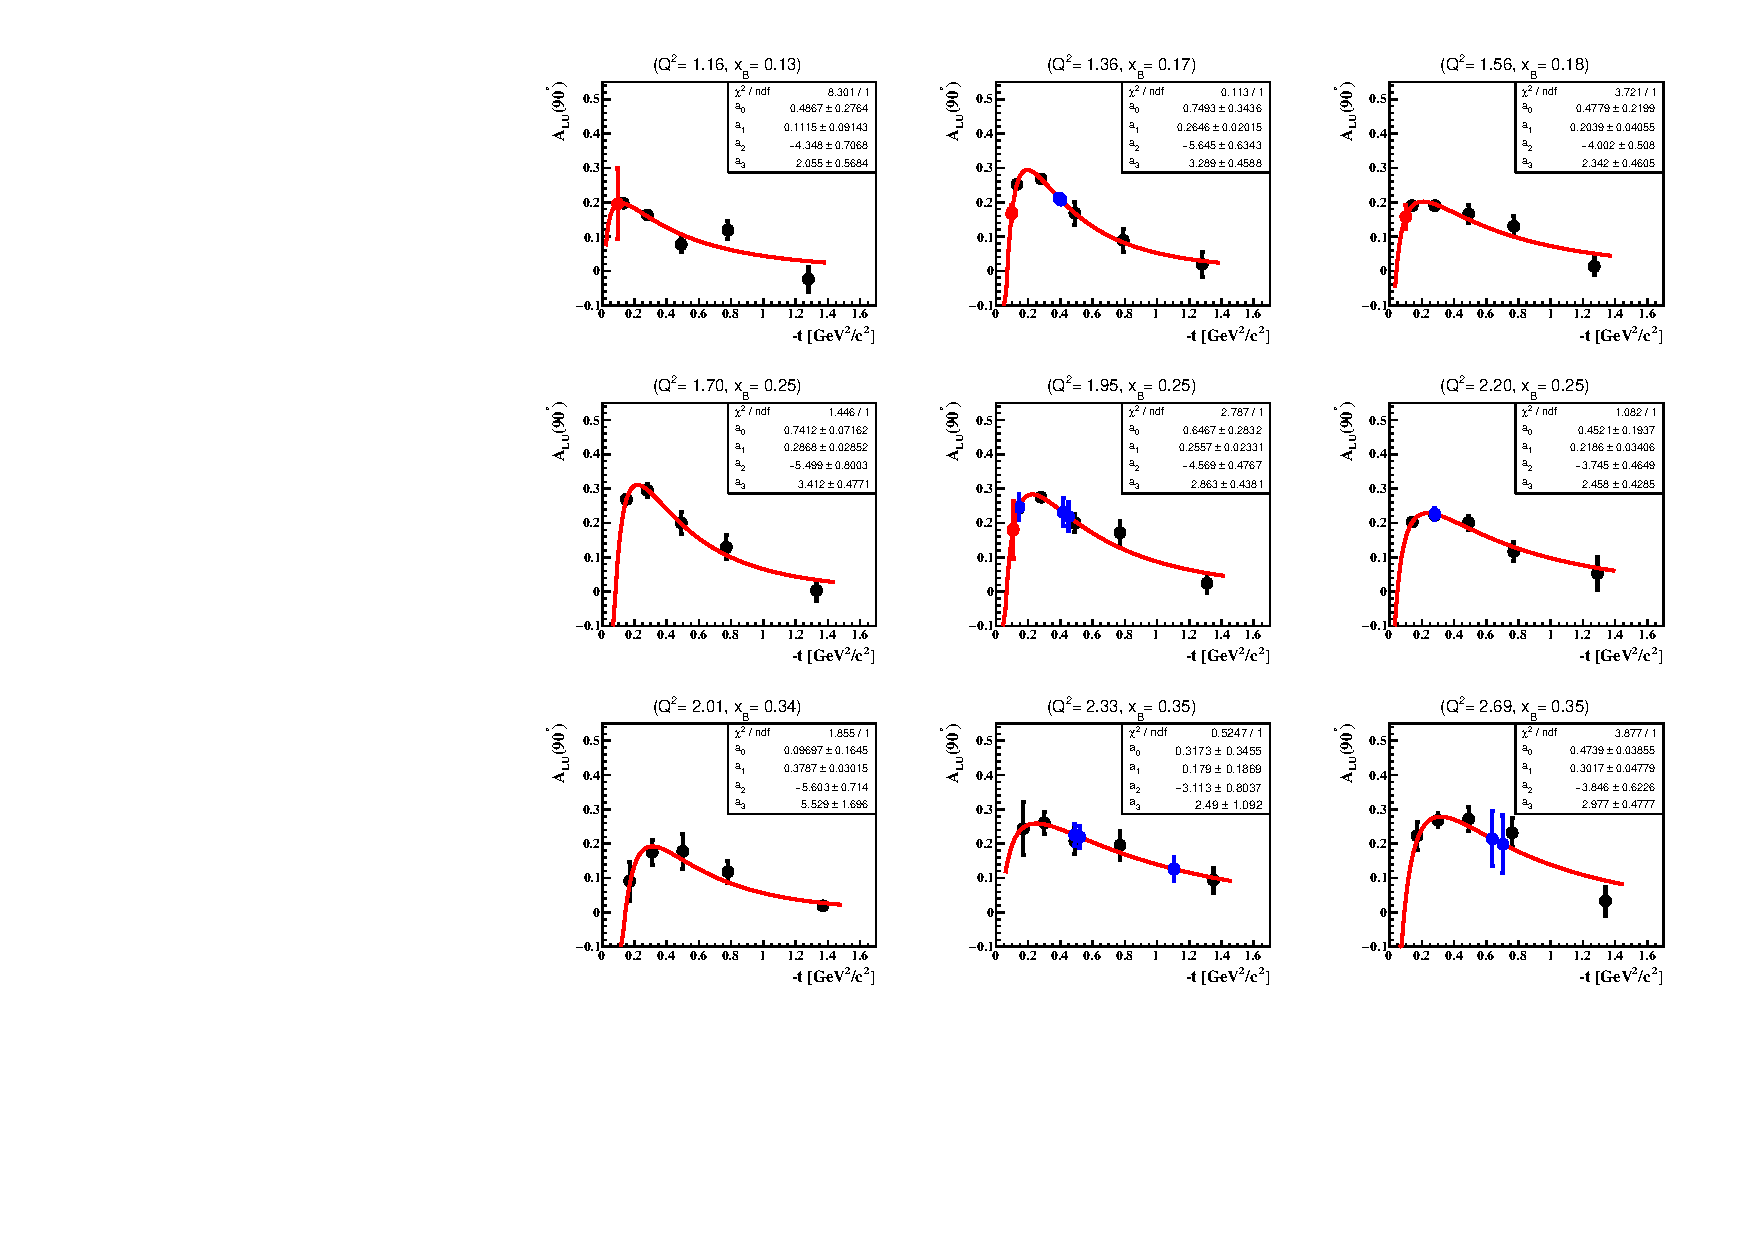
\includegraphics[scale=0.85]{fig_Dec2016/F_ALU-proton-fits.pdf}
\caption{Black circles are the free proton beam-spin asymmetries at $\phi = 90 
   ^{\circ}$ as a function of $-t$ in different ($x_B, Q^2$) bins as measured 
   at CLAS-E1DVCS experiment. The solid red curves are fits to the free proton 
   asymmetries in the form $a_{0}*(\sqrt{t}-a_{1})*e^{a_{2}*\sqrt{t} - a_{3}}$.
   Blue points are the interpolated points corresponding for the incoherent 
points presented in this analysis. The red points stand for the extrapolated 
free proton asymmetries at the measured coherent kinematics.}
\label{fig:free-proton-alu}
\end{figure}


\section{Model-dependent extraction} \label{model_int}
The proton asymmetries have been adjusted using a dispersion calculation 
including a phenomenological GPD $H$ only. The imaginary part of the amplitude 
is parameterized as in \cite{GPD_cal_free_p}. The real part of the amplitude is 
then obtained from the dispersion relation and the D-term as subtraction 
constant, parameterized as in \cite{GPD_cal_free_p}. The beam spin asymmetries 
mostly constrain the parameters of the imaginary part, and the unpolarized 
cross-section mostly constrain the D-term parameters. Figure 
\ref{fig:FXfree-proton-alu} presents the published free proton asymmetries with 
the model calculations, in solid red lines, and the interpolated free proton 
asymmetries at our measured coherent and incoherent kinematic values.

\begin{figure}[tpb]
   \centering
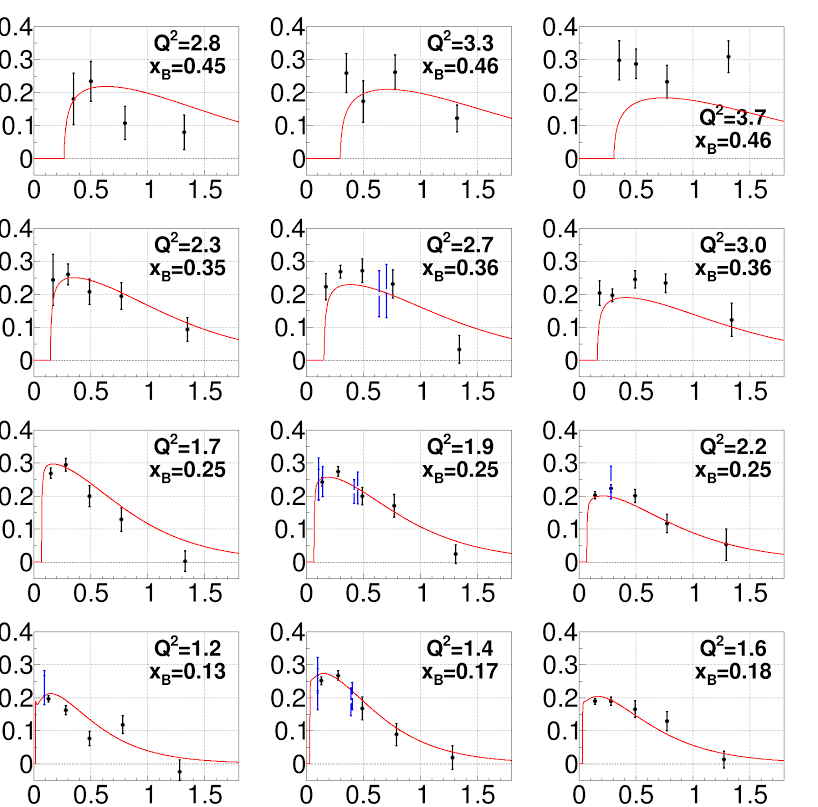
\includegraphics[scale=0.55]{fig_updated/From_FX_Check_Fit_6GeV_asym.png}
\caption{The free proton beam-spin asymmetries at $\phi = 90^{circ}$ as a 
function of $-t$ in different ($x_B, Q^2$) bins as measured at CLAS-E1DVCS 
experiment. The solid red lines are the model calculations based on the 
kinematics of each bin. The blue points stand for the interpolated free proton 
asymmetries at the kinematics of our incoherent DVCS channels.}
\label{fig:FXfree-proton-alu}
\end{figure}

\section{Summary}
In this analysis we use the interpolated values from fitting the experimentally 
measured free proton asymmetries to construct the beam-spin asymmetry ratios, 
presnted in section \ref{fit_int}.  The differences between the beam-spin 
asymmetry ratios calculated using the free proton asymmetries fits, section 
\ref{fit_int}, and the model-dependent interpolated values, section 
\ref{model_int}, were added as a systematic errors on the constructed beam-spin 
asymmetry ratios.  Table \ref{table:ALU_ratios_} presents the coherent and the 
incoherent $A_{LU}$ ratios extracted using both methods and the associated 
systematic uncertainties.

\small
\begin{landscape}
\begin{table}[!h]
   \begin{center}
      \begin{tabular}{||l|l|l|l|l|l||}
         \hline
 ($Q^{2}$, $x_{B}$, $-t$) & EG6 $A_{LU}$ $\pm$ stat. &  Exp. fit $\pm$ stat. & Exp. $A_{LU}$ ratio   &  Model extr. & Model $A_{LU}$ ratio \\
  \hline
 (1.395, 0.166, 0.407) & 0.147 $\pm$ 0.023 & 0.206 $\pm$ 0.009 & 0.715 $\pm$ 0.117 & 0.205 & 0.717 \\
 (1.886, 0.233, 0.499) & 0.153 $\pm$ 0.028 & 0.219 $\pm$ 0.042 & 0.702 $\pm$ 0.188 & 0.224 & 0.683 \\
 (2.338, 0.290, 0.521) & 0.166 $\pm$ 0.032 & 0.219 $\pm$ 0.030 & 0.758 $\pm$ 0.182 & 0.217 & 0.764 \\
 (3.098, 0.379, 0.650) & 0.132 $\pm$ 0.039 & 0.214 $\pm$ 0.080 & 0.619 $\pm$ 0.296 & 0.201 & 0.656 \\
   \hline \hline  \hline                                                                     
 (1.425, 0.162, 0.397) & 0.115 $\pm$ 0.022 & 0.212 $\pm$ 0.009 & 0.545 $\pm$ 0.106 & 0.188 & 0.611 \\
 (1.922, 0.227, 0.418) & 0.182 $\pm$ 0.025 & 0.231 $\pm$ 0.040 & 0.790 $\pm$ 0.176 & 0.213 & 0.854 \\
 (2.354, 0.287, 0.492) & 0.192 $\pm$ 0.030 & 0.225 $\pm$ 0.030 & 0.851 $\pm$ 0.178 & 0.217 & 0.884 \\
 (2.987, 0.390, 0.714) & 0.149 $\pm$ 0.046 & 0.198 $\pm$ 0.083 & 0.754 $\pm$ 0.396 & 0.210 & 0.709 \\
   \hline  \hline  \hline                                                                    
 (1.823, 0.213, 0.145) & 0.142 $\pm$ 0.023 & 0.246 $\pm$ 0.037 & 0.576 $\pm$ 0.131 & 0.243 & 0.584 \\
 (2.127, 0.255, 0.282) & 0.155 $\pm$ 0.027 & 0.225 $\pm$ 0.018 & 0.688 $\pm$ 0.131 & 0.241 & 0.643 \\
 (2.308, 0.284, 0.490) & 0.183 $\pm$ 0.034 & 0.225 $\pm$ 0.030 & 0.811 $\pm$ 0.188 & 0.219 & 0.835 \\
 (2.406, 0.308, 1.107) & 0.170 $\pm$ 0.051 & 0.126 $\pm$ 0.034 & 1.343 $\pm$ 0.545 & 0.123 & 1.382 \\
   \hline  \hline  \hline                                                                    
 (1.143, 0.132, 0.096) & 0.303 $\pm$ 0.051 & 0.195 $\pm$ 0.102 & 1.552 $\pm$ 0.857 & 0.244 & 1.241 \\
 (1.423, 0.170, 0.099) & 0.364 $\pm$ 0.059 & 0.170 $\pm$ 0.020 & 2.137 $\pm$ 0.431 & 0.251 & 1.450 \\
 (1.902, 0.224, 0.107) & 0.294 $\pm$ 0.060 & 0.181 $\pm$ 0.082 & 1.624 $\pm$ 0.808 & 0.235 & 1.251 \\
     \hline \hline  \hline                                                                   
 (1.164, 0.132, 0.095) & 0.319 $\pm$ 0.044 & 0.195 $\pm$ 0.102 & 1.633 $\pm$ 0.888 & 0.223 & 1.430 \\
 (1.439, 0.170, 0.099) & 0.278 $\pm$ 0.078 & 0.166 $\pm$ 0.020 & 1.670 $\pm$ 0.518 & 0.243 & 1.144 \\
 (1.844, 0.225, 0.107) & 0.319 $\pm$ 0.161 & 0.178 $\pm$ 0.084 & 1.788 $\pm$ 1.235 & 0.251 & 1.270 \\
      \hline  \hline  \hline                                                                 
 (1.493, 0.177, 0.1)   & 0.349 $\pm$ 0.029 & 0.157 $\pm$ 0.034 & 2.214 $\pm$ 0.515 & 0.245 & 1.424 \\                                                               
 \hline
 \end{tabular}
 \caption{$A_{LU}$ ratios. The first three blocks stand for the incoherent bins 
 in $Q^{2}$, $x_{B}$, and $-t$, respectively. The last three blocks are for the 
 coherent bins in $Q^{2}$, $x_{B}$, and $-t$, respectively. The first column 
 contains the mean value of the kinematical variables for each bin. The second 
 column contains EG6 measured $A_{LU}$ with the statistical error bars. The 
 third column ("Exp. fit $\pm$ stat.") contains the interpolated free proton 
 $A_{LU}$ at EG6 kinematical values from fitting the free proton beam-spin 
 asymmetries. The forth column ("Exp. $A_{LU}$ ratio") stands for the 
 calculated $A_{LU}$ ratios using EG6 asymmetries and the fitted free proton 
 asymmetries. The fifth column ("Model extr.") stands for the model-depended 
 extracted free proton asymmetries. The sixth column ("Model $A_{LU}$ ratio") 
 presents the calculated $A_{LU}$ ratios using EG6 asymmetries and the 
 model-dependent extracted free proton asymmetries. }
 \label{table:ALU_ratios_}
 \end{center}
\end{table}
\end{landscape}





